\documentclass[a4paper]{article}
% Cấu hình lề và kích thước Header/Footer
\usepackage[a4paper, margin=2cm, headheight=45pt, footskip=1.2cm]{geometry}
\usepackage[utf8]{inputenc}
\usepackage[T5]{fontenc} 
\usepackage[vietnamese]{babel}
\usepackage{amsmath, amssymb, amsfonts}
\usepackage{graphicx}
\usepackage{xcolor}
\usepackage{tikz}
\usepackage{pgfplots}
\pgfplotsset{compat=1.18}
\usetikzlibrary{shapes.geometric, arrows.meta, positioning, fit, backgrounds}
\usepackage{listings}
\usepackage{booktabs, array, multirow, colortbl}
\usepackage{float}
\usepackage{fancyhdr}
\usepackage{lastpage}
\usepackage[hidelinks]{hyperref}

% ===================== CODE STYLE PYTHON =====================
\definecolor{codebg}{RGB}{245,245,245}
\definecolor{codeframe}{RGB}{200,200,200}
\definecolor{keyword}{RGB}{0,0,180}
\definecolor{comment}{RGB}{80,120,80}
\definecolor{string}{RGB}{160,30,30}

\lstdefinestyle{pythonstyle}{
    backgroundcolor=\color{codebg},
    frame=single,
    rulecolor=\color{codeframe},
    basicstyle=\ttfamily\small,
    keywordstyle=\color{keyword}\bfseries,
    commentstyle=\color{comment}\itshape,
    stringstyle=\color{string},
    numberstyle=\tiny\color{gray},
    numbers=left,
    numbersep=8pt,
    tabsize=4,
    showstringspaces=false,
    breaklines=true,
    captionpos=b,
    language=Python,
    extendedchars=true,
    literate=
        {á}{{\'a}}1 {à}{{\`a}}1 {ả}{{\h{a}}}1 {ã}{{\~a}}1 {ạ}{{\d{a}}}1
        {ă}{{\u{a}}}1 {ắ}{{\'\u{a}}}1 {ằ}{{\`\u{a}}}1 {ẳ}{{\h{\u{a}}}}1
        {ẵ}{{\~\u{a}}}1 {ặ}{{\d{\u{a}}}}1
        {â}{{\^a}}1 {ấ}{{\'\^a}}1 {ầ}{{\`\^a}}1 {ẩ}{{\h{\^a}}}1
        {ẫ}{{\~\^a}}1 {ậ}{{\d{\^a}}}1
        {é}{{\'e}}1 {è}{{\`e}}1 {ẻ}{{\h{e}}}1 {ẽ}{{\~e}}1 {ẹ}{{\d{e}}}1
        {ê}{{\^e}}1 {ế}{{\'\^e}}1 {ề}{{\`\^e}}1 {ể}{{\h{\^e}}}1
        {ễ}{{\~\^e}}1 {ệ}{{\d{\^e}}}1
        {í}{{\'i}}1 {ì}{{\`i}}1 {ỉ}{{\h{i}}}1 {ĩ}{{\~i}}1 {ị}{{\d{i}}}1
        {ó}{{\'o}}1 {ò}{{\`o}}1 {ỏ}{{\h{o}}}1 {õ}{{\~o}}1 {ọ}{{\d{o}}}1
        {ô}{{\^o}}1 {ố}{{\'\^o}}1 {ồ}{{\`\^o}}1 {ổ}{{\h{\^o}}}1
        {ỗ}{{\~\^o}}1 {ộ}{{\d{\^o}}}1
        {ơ}{{\horn{o}}}1 {ớ}{{\'\horn{o}}}1 {ờ}{{\`\horn{o}}}1
        {ở}{{\h{\horn{o}}}}1 {ỡ}{{\~\horn{o}}}1 {ợ}{{\d{\horn{o}}}}1
        {ú}{{\'u}}1 {ù}{{\`u}}1 {ủ}{{\h{u}}}1 {ũ}{{\~u}}1 {ụ}{{\d{u}}}1
        {ư}{{\horn{u}}}1 {ứ}{{\'\horn{u}}}1 {ừ}{{\`\horn{u}}}1
        {ử}{{\h{\horn{u}}}}1 {ữ}{{\~\horn{u}}}1 {ự}{{\d{\horn{u}}}}1
        {ý}{{\'y}}1 {ỳ}{{\`y}}1 {ỷ}{{\h{y}}}1 {ỹ}{{\~y}}1 {ỵ}{{\d{y}}}1
        {đ}{{\dj}}1 {Đ}{{\DJ}}1
}
% ---------- GHI CHÚ PHẦN CHƯA HOÀN THÀNH ----------
% Dùng \todo{...} cho các phần chờ kết quả thực nghiệm; xóa khi đã điền số liệu.
\newcommand{\todo}[1]{\colorbox{yellow!40}{\parbox{0.95\linewidth}{\small\textbf{TODO:} #1}}}

% ---------- HEADER & FOOTER CONFIGURATION ----------
\pagestyle{fancy}
\fancyhf{}

\fancyhead[L]{
 \begin{tabular}{rl}
    \begin{picture}(25,15)(0,0)
    \put(-3,-14){
\includegraphics[width=17mm]{hcmut.png}}
   \end{picture}&
    \begin{tabular}{l}
        \textbf{\ttfamily TRƯỜNG ĐẠI HỌC BÁCH KHOA - ĐHQG-HCM}\\
        \textbf{\ttfamily KHOA KHOA HỌC VÀ KỸ THUẬT MÁY TÍNH}
    \end{tabular}
 \end{tabular}
}

\fancyfoot[L]{\scriptsize \ttfamily Lập trình cho TTNT và KHDL (CO3135) - HK261 - Năm học 2026-2027}
\fancyfoot[R]{\scriptsize \ttfamily Trang {\thepage}/\pageref{LastPage}}

\renewcommand{\headrulewidth}{0.3pt}
\renewcommand{\footrulewidth}{0.3pt}

\linespread{1.5}
\setlength{\emergencystretch}{3em} % tránh tràn lề với các đoạn \texttt dài

\begin{document}

% Trang bìa
\begin{titlepage}
\begin{center}
VIETNAM NATIONAL UNIVERSITY, HO CHI MINH CITY \\
UNIVERSITY OF TECHNOLOGY \\
FACULTY OF COMPUTER SCIENCE AND ENGINEERING
\end{center}
\vspace{1cm}
\begin{figure}[h!]
\begin{center}

\includegraphics[width=10cm]{hcmut.png}
\end{center}
\end{figure}
\vspace{0.5cm}
\begin{center}
\begin{tabular}{c}
\multicolumn{1}{l}{\textbf{{\Large Lập trình cho Trí tuệ nhân tạo và Khoa học dữ liệu (CO3135)}}}\\
\multicolumn{1}{l}{\textbf{{\large HK261 - Lớp L01}}}\\
~~\\ \hline \\
\multicolumn{1}{l}{\textbf{{\Large Bài tập lớn}}}\\ \\
\parbox{15cm}{\centering\textbf{\textit{{\LARGE Dự đoán khách hàng rời đi bằng máy học với kỹ thuật xử lý đặc trưng và tối ưu hóa siêu tham số}}}}\\ \\ \hline
\end{tabular}
\end{center}
\vspace{1.5cm}
\begin{table}[h]
\centering
    \begin{tabular}{rl}
    \hspace{3 cm}\textbf{Giảng viên hướng dẫn}: & Trần Huy\\
    & \\[10pt]
    \textbf{Sinh viên thực hiện}:
    & Nguyễn Tiến Bách - 2310201\\
    & Trần Gia Bảo Anh - 2310148\\
    \end{tabular}
\end{table}
\vfill
\begin{center}
{\footnotesize HO CHI MINH CITY, NOVEMBER 2026}
\end{center}
\end{titlepage}

% Trang mục lục
\newpage
\tableofcontents
\thispagestyle{fancy}
\newpage

% Các nội dung chính
\section{Giới thiệu đề tài}

\subsection{Đặt vấn đề}
Trong các ngành dịch vụ thuê bao như viễn thông, ngân hàng hay các nền tảng trực tuyến, \textbf{khách hàng rời bỏ} (\textit{customer churn}) là một trong những nguyên nhân chính làm suy giảm doanh thu. Chi phí để thu hút một khách hàng mới thường cao hơn nhiều so với chi phí giữ chân một khách hàng hiện tại, vì vậy doanh nghiệp có động lực lớn để nhận diện sớm những khách hàng có nguy cơ rời bỏ và chủ động đưa ra các chính sách giữ chân (ưu đãi, nâng cấp hợp đồng, hỗ trợ kỹ thuật,\ldots).

Khách hàng có thể ngừng sử dụng dịch vụ vì chi phí cao, chất lượng dịch vụ không phù hợp, hợp đồng ngắn hạn dễ chấm dứt hoặc nhiều lý do khác. Các dấu hiệu này thường ẩn trong thông tin hợp đồng, lịch sử sử dụng và hành vi thanh toán của khách hàng. Đây là bối cảnh phù hợp để ứng dụng các thuật toán Học máy (Machine Learning) nhằm khai thác các quy luật từ dữ liệu lịch sử.

\subsection{Phát biểu bài toán}
Dựa trên thông tin nhân khẩu học, các dịch vụ đã đăng ký, thông tin hợp đồng và chi phí của khách hàng, bài toán đặt ra là dự đoán khách hàng đó có rời bỏ dịch vụ hay không. Đây là bài toán \textbf{phân loại nhị phân} (\textit{binary classification}):
\begin{itemize}
    \item \textbf{Đầu vào:} vector đặc trưng $\mathbf{x}$ gồm 19 thuộc tính của một khách hàng (giới tính, thời gian sử dụng, loại hợp đồng, phương thức thanh toán, chi phí hàng tháng,\ldots).
    \item \textbf{Đầu ra:} nhãn $y \in \{0, 1\}$, trong đó
    \begin{itemize}
        \item $\text{Churn} = 0$: khách hàng không rời bỏ dịch vụ;
        \item $\text{Churn} = 1$: khách hàng rời bỏ dịch vụ.
    \end{itemize}
\end{itemize}
Ngoài nhãn dự đoán, mô hình còn cung cấp xác suất $P(y=1 \mid \mathbf{x})$, cho phép doanh nghiệp xếp hạng khách hàng theo mức độ rủi ro và ưu tiên nguồn lực giữ chân.

\subsection{Mục tiêu}
Đề tài tập trung vào nhánh \textbf{Classic Machine Learning} với các mục tiêu cụ thể:
\begin{enumerate}
    \item Xây dựng một \textbf{pipeline} học máy hoàn chỉnh, có thể tái lập, từ đọc dữ liệu, làm sạch, tiền xử lý đến huấn luyện, đánh giá và dự đoán cho khách hàng mới.
    \item Huấn luyện và so sánh bốn thuật toán: Logistic Regression, Decision Tree, Random Forest và XGBoost.
    \item Đánh giá ảnh hưởng của \textbf{Feature Engineering}, kỹ thuật \textbf{xử lý mất cân bằng dữ liệu}, \textbf{Hyperparameter Tuning} và việc \textbf{chọn ngưỡng quyết định} lên hiệu năng mô hình.
    \item Giải thích mô hình (permutation importance, hệ số Logistic Regression) và liên hệ kết quả với góc nhìn kinh doanh. Các mối liên hệ rút ra là quan hệ thống kê quan sát được từ dữ liệu, không phải kết luận nhân quả.
\end{enumerate}

\subsection{Phạm vi và phương pháp thực hiện}
Đề tài sử dụng bộ dữ liệu công khai \textit{Telco Customer Churn} của IBM (7.043 khách hàng, 21 cột). Quy trình được triển khai theo các bước:
\begin{itemize}
    \item \textbf{Khám phá và làm sạch dữ liệu (EDA):} kiểm tra kiểu dữ liệu, giá trị thiếu, trùng lặp, phân bố nhãn và mối liên hệ giữa các đặc trưng với Churn.
    \item \textbf{Tiền xử lý:} xử lý giá trị thiếu, One-Hot Encoding cho biến phân loại, chuẩn hóa biến số khi cần, chia Train/Test 80/20 có phân tầng (\textit{stratified}).
    \item \textbf{Feature Engineering:} tạo các đặc trưng mới như nhóm thời gian sử dụng, số dịch vụ đăng ký, đặc trưng kết hợp hợp đồng -- thời gian -- chi phí.
    \item \textbf{Huấn luyện và tối ưu:} Stratified 5-fold Cross-Validation trên tập train; tối ưu siêu tham số bằng RandomizedSearchCV; chọn ngưỡng quyết định trên xác suất out-of-fold.
    \item \textbf{Đánh giá:} Accuracy, Precision, Recall, F1-score, ROC-AUC, PR-AUC và Confusion Matrix trên tập test được giữ riêng.
\end{itemize}

Toàn bộ dự án được cài đặt bằng Python với các thư viện \texttt{pandas}, \texttt{numpy}, \texttt{scikit-learn}, \texttt{xgboost}, \texttt{matplotlib} và \texttt{seaborn}. Bài toán không yêu cầu GPU hay Deep Learning.

\subsection{Link github (Source Code)}
\url{https://github.com/BachNguyen0710/AI-KHDL-assignment}

\section{Tổng quan tài liệu}

\subsection{Bài toán dự đoán khách hàng rời bỏ}
Dự đoán khách hàng rời bỏ là một bài toán kinh điển trong quản trị quan hệ khách hàng (CRM), đặc biệt trong ngành viễn thông -- nơi thị trường bão hòa và chi phí chuyển đổi nhà mạng thấp. Các nghiên cứu thường mô hình hóa bài toán dưới dạng phân loại nhị phân có giám sát trên dữ liệu dạng bảng (\textit{tabular data}) gồm thông tin hợp đồng, hành vi sử dụng và thanh toán \cite{huang2012, verbeke2012}.

Một số đặc điểm chung của bài toán được ghi nhận trong tài liệu:
\begin{itemize}
    \item \textbf{Dữ liệu mất cân bằng:} số khách hàng rời bỏ thường chiếm thiểu số, khiến Accuracy dễ gây hiểu lầm; các chỉ số như Recall, F1-score, ROC-AUC được ưu tiên \cite{vafeiadis2015}.
    \item \textbf{Chi phí sai sót không đối xứng:} bỏ sót một khách hàng sắp rời bỏ (False Negative) thường tốn kém hơn việc gửi nhầm ưu đãi cho khách hàng trung thành (False Positive). Verbeke và cộng sự \cite{verbeke2012} đề xuất đánh giá mô hình theo lợi nhuận kỳ vọng thay vì chỉ theo độ chính xác.
    \item \textbf{Vai trò của đặc trưng:} chất lượng đặc trưng đầu vào ảnh hưởng mạnh đến hiệu năng; nhiều nghiên cứu cho thấy Feature Engineering dựa trên hiểu biết nghiệp vụ mang lại cải thiện đáng kể \cite{huang2012, ahmad2019}.
\end{itemize}

\subsection{Các phương pháp học máy cổ điển}

\subsubsection{Logistic Regression}
Logistic Regression là mô hình tuyến tính tổng quát ước lượng xác suất thuộc lớp dương thông qua hàm sigmoid \cite{hosmer2013}:
\begin{equation}
    P(y = 1 \mid \mathbf{x}) = \sigma(\mathbf{w}^\top \mathbf{x} + b) = \frac{1}{1 + e^{-(\mathbf{w}^\top \mathbf{x} + b)}}
\end{equation}
Tham số được học bằng cách cực tiểu hóa hàm mất mát log-loss có chính quy hóa:
\begin{equation}
    \mathcal{L}(\mathbf{w}, b) = -\frac{1}{n}\sum_{i=1}^{n}\left[y_i \log \hat{p}_i + (1-y_i)\log(1-\hat{p}_i)\right] + \frac{1}{2C}\|\mathbf{w}\|_2^2
\end{equation}
trong đó $C$ là nghịch đảo cường độ chính quy hóa. Ưu điểm: nhanh, ổn định, hệ số dễ diễn giải; thường là \textit{baseline} mạnh trên dữ liệu churn. Nhược điểm: chỉ biểu diễn được biên quyết định tuyến tính, nhạy với thang đo của đặc trưng nên cần chuẩn hóa.

\subsubsection{Decision Tree}
Cây quyết định (CART \cite{breiman1984}) chia không gian đặc trưng thành các vùng bằng chuỗi luật \textit{if--then}. Tại mỗi nút, thuật toán chọn đặc trưng và ngưỡng làm giảm nhiều nhất độ vẩn đục, ví dụ chỉ số Gini:
\begin{equation}
    \text{Gini}(S) = 1 - \sum_{k=1}^{K} p_k^2
\end{equation}
Cây dễ diễn giải, không cần chuẩn hóa và tự nắm bắt được tương tác phi tuyến, nhưng có phương sai cao: nếu không giới hạn \texttt{max\_depth}, \texttt{min\_samples\_split},\ldots, cây dễ học thuộc dữ liệu huấn luyện (\textit{overfitting}).

\subsubsection{Random Forest}
Random Forest \cite{breiman2001} là phương pháp \textit{ensemble} theo hướng \textit{bagging}: huấn luyện $T$ cây trên các mẫu bootstrap khác nhau, mỗi lần tách nút chỉ xét một tập con ngẫu nhiên các đặc trưng, rồi tổng hợp bằng bỏ phiếu/trung bình xác suất:
\begin{equation}
    \hat{p}(\mathbf{x}) = \frac{1}{T}\sum_{t=1}^{T} h_t(\mathbf{x})
\end{equation}
Việc lấy trung bình nhiều cây ít tương quan giúp giảm phương sai so với một cây đơn lẻ, nhờ đó Random Forest thường có hiệu năng tốt và ổn định trên dữ liệu bảng.

\subsubsection{Gradient Boosting và XGBoost}
Khác với bagging, \textit{boosting} xây dựng các cây tuần tự, mỗi cây mới học phần sai số (gradient) của mô hình hiện tại:
\begin{equation}
    F_m(\mathbf{x}) = F_{m-1}(\mathbf{x}) + \eta \, h_m(\mathbf{x})
\end{equation}
với $\eta$ là tốc độ học (\texttt{learning\_rate}). XGBoost \cite{chen2016} bổ sung xấp xỉ bậc hai của hàm mất mát, chính quy hóa độ phức tạp cây, xử lý giá trị thiếu và nhiều tối ưu tính toán. XGBoost là một trong những thuật toán mạnh nhất cho dữ liệu dạng bảng, nhưng có nhiều siêu tham số và dễ overfit nếu không được tinh chỉnh.

\subsubsection{Các nghiên cứu so sánh}
Vafeiadis và cộng sự \cite{vafeiadis2015} so sánh nhiều thuật toán (mạng nơ-ron, SVM, cây quyết định, Naïve Bayes, Logistic Regression) cho bài toán churn viễn thông và cho thấy việc kết hợp boosting giúp cải thiện hiệu năng, trong đó SVM kết hợp boosting đạt kết quả tốt nhất. Ahmad và cộng sự \cite{ahmad2019} xây dựng hệ thống dự đoán churn trên nền tảng dữ liệu lớn và ghi nhận XGBoost cho AUC cao nhất trong các mô hình được thử nghiệm. Nhìn chung, các phương pháp ensemble dựa trên cây thường vượt trội, tuy nhiên mức chênh lệch phụ thuộc mạnh vào dữ liệu, đặc trưng và việc tinh chỉnh siêu tham số -- đây là lý do đề tài so sánh các mô hình trên cùng một quy trình đánh giá.

\subsection{Tiền xử lý và Feature Engineering}
\begin{itemize}
    \item \textbf{Mã hóa biến phân loại:} One-Hot Encoding phù hợp với biến danh nghĩa có ít giá trị; Ordinal/Label Encoding gọn hơn và phù hợp cho mô hình cây; Target Encoding hữu ích khi số giá trị lớn nhưng cần thực hiện trong từng fold để tránh rò rỉ nhãn.
    \item \textbf{Chuẩn hóa:} StandardScaler, MinMaxScaler, RobustScaler cần thiết cho các mô hình dựa trên khoảng cách hoặc gradient (Logistic Regression), nhưng không ảnh hưởng đến mô hình cây.
    \item \textbf{Feature Engineering:} tạo đặc trưng từ hiểu biết nghiệp vụ, ví dụ nhóm thời gian gắn bó, tổng số dịch vụ sử dụng, chi phí trung bình mỗi tháng hay các đặc trưng tương tác giữa loại hợp đồng và chi phí.
    \item \textbf{Tránh rò rỉ dữ liệu:} mọi bước \texttt{fit} của tiền xử lý phải được thực hiện chỉ trên phần dữ liệu huấn luyện; trong \texttt{scikit-learn} \cite{pedregosa2011} điều này được đảm bảo bằng cách đóng gói tiền xử lý và mô hình trong một \texttt{Pipeline}.
\end{itemize}

\subsection{Xử lý mất cân bằng dữ liệu}
\begin{itemize}
    \item \textbf{Class weight / cost-sensitive learning:} gán trọng số lớn hơn cho lớp thiểu số trong hàm mất mát (\texttt{class\_weight="balanced"} hoặc \texttt{scale\_pos\_weight} trong XGBoost).
    \item \textbf{SMOTE} \cite{chawla2002}: sinh mẫu tổng hợp cho lớp thiểu số bằng nội suy giữa một mẫu và các láng giềng gần nhất cùng lớp. SMOTE chỉ được áp dụng trên phần huấn luyện của mỗi fold.
    \item \textbf{Điều chỉnh ngưỡng quyết định:} thay vì ngưỡng 0{,}5 mặc định, chọn ngưỡng trên tập validation để cân bằng Precision và Recall theo mục tiêu kinh doanh.
\end{itemize}

\subsection{Tối ưu siêu tham số}
\begin{itemize}
    \item \textbf{Grid Search:} thử toàn bộ tổ hợp trên lưới rời rạc; đơn giản nhưng chi phí tăng theo cấp số nhân với số siêu tham số.
    \item \textbf{Random Search} \cite{bergstra2012}: lấy mẫu ngẫu nhiên trong không gian tìm kiếm; với cùng ngân sách thường hiệu quả hơn Grid Search khi chỉ một số ít siêu tham số thực sự quan trọng.
    \item \textbf{Tối ưu Bayes / Optuna} \cite{akiba2019}: dùng kết quả các lần thử trước (ví dụ thuật toán TPE) để đề xuất cấu hình tiếp theo, kết hợp cơ chế cắt tỉa (\textit{pruning}) các lần thử kém.
\end{itemize}

\subsection{Giải thích mô hình}
Bên cạnh \textit{feature importance} của mô hình cây và hệ số của Logistic Regression, SHAP (SHapley Additive exPlanations) \cite{lundberg2017} phân rã mỗi dự đoán thành tổng đóng góp của từng đặc trưng dựa trên giá trị Shapley của lý thuyết trò chơi:
\begin{equation}
    f(\mathbf{x}) = \phi_0 + \sum_{j=1}^{M} \phi_j
\end{equation}
SHAP cho phép giải thích cả ở mức toàn cục (đặc trưng nào quan trọng nhất) và mức từng khách hàng (vì sao một khách hàng bị dự đoán có nguy cơ cao).

Một cách đơn giản hơn và không phụ thuộc mô hình là \textbf{permutation importance}, được đề xuất cùng Random Forest \cite{breiman2001}: xáo trộn ngẫu nhiên giá trị của một đặc trưng trên tập đánh giá và đo mức giảm của chỉ số đánh giá. Đặc trưng làm chỉ số giảm càng nhiều thì mô hình càng dựa vào nó. Cách này đo trực tiếp trên đặc trưng gốc (trước One-Hot Encoding) nên dễ diễn giải, nhưng có thể đánh giá thấp các đặc trưng tương quan mạnh với nhau.

\subsection{Định hướng của đề tài}
Từ khảo sát trên, đề tài lựa chọn so sánh bốn mô hình đại diện cho các họ thuật toán khác nhau (tuyến tính, cây đơn, bagging, boosting) trên cùng một pipeline và cùng cách chia dữ liệu, đồng thời lần lượt đánh giá đóng góp của từng kỹ thuật: Feature Engineering, xử lý mất cân bằng, Hyperparameter Tuning và chọn ngưỡng quyết định.

\section{Dữ liệu và tiền xử lý}

\subsection{Mô tả bộ dữ liệu}
Đề tài sử dụng bộ dữ liệu \textbf{Telco Customer Churn} do IBM công bố, được chia sẻ công khai trên Kaggle\footnote{\url{https://www.kaggle.com/datasets/blastchar/telco-customer-churn}}. Bộ dữ liệu gồm \textbf{7.043 khách hàng} và \textbf{21 cột}: một mã định danh \texttt{customerID}, 19 đặc trưng đầu vào và nhãn mục tiêu \texttt{Churn}.

\begin{table}[H]
\centering
\begin{tabular}{p{4cm} p{8.5cm} l}
\toprule
\textbf{Nhóm thông tin} & \textbf{Các cột} & \textbf{Kiểu} \\
\midrule
Nhân khẩu học & \texttt{gender}, \texttt{SeniorCitizen}, \texttt{Partner}, \texttt{Dependents} & Phân loại / nhị phân \\
Dịch vụ & \texttt{PhoneService}, \texttt{MultipleLines}, \texttt{InternetService}, \texttt{OnlineSecurity}, \texttt{OnlineBackup}, \texttt{DeviceProtection}, \texttt{TechSupport}, \texttt{StreamingTV}, \texttt{StreamingMovies} & Phân loại \\
Hợp đồng, thanh toán & \texttt{Contract}, \texttt{PaperlessBilling}, \texttt{PaymentMethod} & Phân loại \\
Chi phí & \texttt{MonthlyCharges}, \texttt{TotalCharges} & Số thực \\
Thời gian sử dụng & \texttt{tenure} (tháng) & Số nguyên \\
Nhãn & \texttt{Churn} (Yes/No) & Nhị phân \\
\bottomrule
\end{tabular}
\caption{Các nhóm thuộc tính trong bộ dữ liệu Telco Customer Churn}
\end{table}

\subsection{Kiểm tra chất lượng dữ liệu}
Quá trình khám phá dữ liệu được thực hiện trong notebook \texttt{01\_eda.ipynb} và được đóng gói lại thành hàm \texttt{load\_and\_clean\_data()} trong \texttt{src/data.py}. Các kết quả kiểm tra chính:
\begin{itemize}
    \item Không có dòng trùng lặp; \texttt{customerID} không thiếu và không trùng.
    \item Cột \texttt{TotalCharges} được đọc dưới dạng chuỗi và chứa \textbf{11 giá trị chỉ gồm khoảng trắng}. Các giá trị này được chuyển thành giá trị thiếu (NaN), sau đó cột được ép sang kiểu số. Ngoài 11 trường hợp này không có giá trị nào không thể chuyển thành số.
    \item Cả 11 khách hàng thiếu \texttt{TotalCharges} đều có \texttt{tenure} $= 0$, tức là khách hàng mới chưa phát sinh hóa đơn. Nhóm quyết định không thay cứng bằng 0 mà để bước \textit{imputation} trong pipeline xử lý.
    \item Không có giá trị âm. \texttt{tenure} nằm trong khoảng 0--72 tháng; \texttt{MonthlyCharges} trong khoảng 18{,}25--118{,}75; \texttt{TotalCharges} trong khoảng 18{,}80--8.684{,}80.
    \item Các giá trị \textit{``No internet service''} và \textit{``No phone service''} phản ánh tình trạng sử dụng dịch vụ, không phải giá trị thiếu, nên được giữ nguyên như một hạng mục riêng.
\end{itemize}

Hàm làm sạch kiểm tra chặt chẽ các điều kiện trên và báo lỗi nếu dữ liệu đầu vào không hợp lệ:

\begin{lstlisting}[style=pythonstyle, caption={Làm sạch TotalCharges và mã hóa nhãn trong \texttt{src/data.py}}]
for column in text_columns:
    df[column] = df[column].str.strip().replace("", float("nan"))

total_charges = pd.to_numeric(df["TotalCharges"], errors="coerce")
invalid_values = df["TotalCharges"].notna() & total_charges.isna()
if invalid_values.any():
    raise ValueError("TotalCharges contains non-numeric values")
df["TotalCharges"] = total_charges

df["Churn"] = df["Churn"].map({"No": 0, "Yes": 1})
\end{lstlisting}

\subsection{Phân bố nhãn và chia dữ liệu}
Trên toàn bộ dữ liệu có 5.174 khách hàng không rời bỏ (73{,}46\%) và 1.869 khách hàng rời bỏ (26{,}54\%). Dữ liệu \textbf{mất cân bằng ở mức vừa phải} (tỉ lệ xấp xỉ 2{,}8 : 1), vì vậy Accuracy không được dùng làm chỉ số duy nhất.

Dữ liệu được chia \textbf{Train/Test theo tỉ lệ 80/20} bằng \texttt{train\_test\_split} với \texttt{stratify=Churn} và \texttt{random\_state=42}:
\begin{itemize}
    \item Train: 5.634 khách hàng (tỉ lệ churn 26{,}54\%).
    \item Test: 1.409 khách hàng (tỉ lệ churn 26{,}54\%).
\end{itemize}
Danh sách \texttt{customerID} của mỗi tập được lưu vào \texttt{data/splits/train\_ids.csv} và \texttt{test\_ids.csv}. Mọi thực nghiệm sau đó đều đọc lại đúng hai danh sách này, đảm bảo \textbf{cùng một cách chia dữ liệu} cho mọi mô hình. Tập test được giữ riêng hoàn toàn, chỉ dùng cho đánh giá cuối cùng; mọi phân tích EDA chuyên sâu và lựa chọn mô hình đều thực hiện trên tập train.

\begin{figure}[H]
\centering
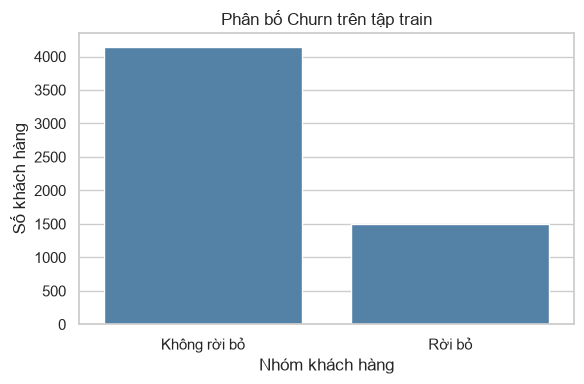
\includegraphics[width=0.5\textwidth]{img/eda_churn_distribution.png}
\caption{Phân bố nhãn Churn trên tập train}
\end{figure}

\subsection{Phân tích khám phá (EDA)}\label{sec:eda}

\subsubsection{Đặc trưng số}
\begin{figure}[H]
\centering
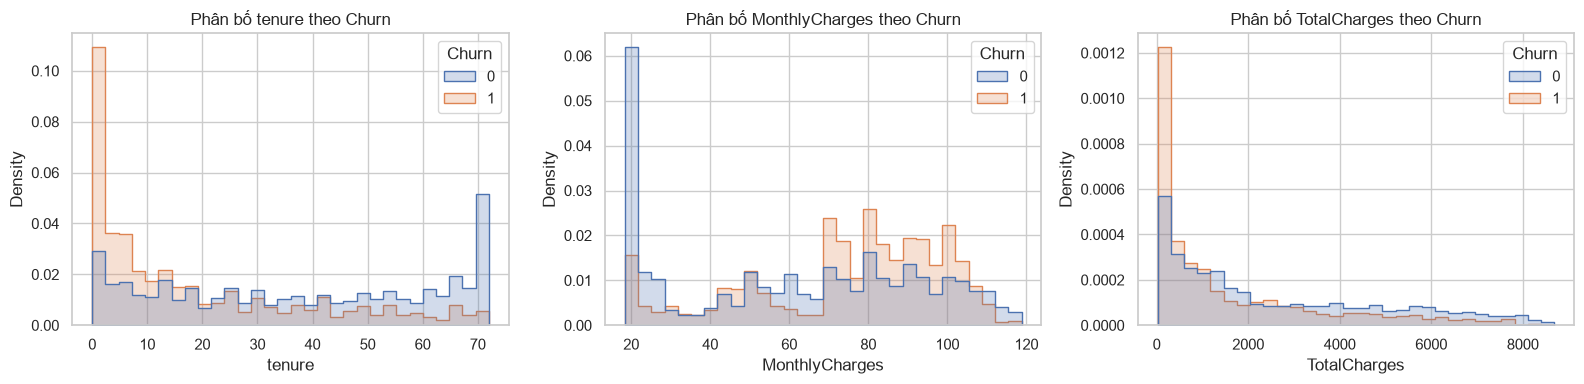
\includegraphics[width=\textwidth]{img/eda_numeric_hist.png}
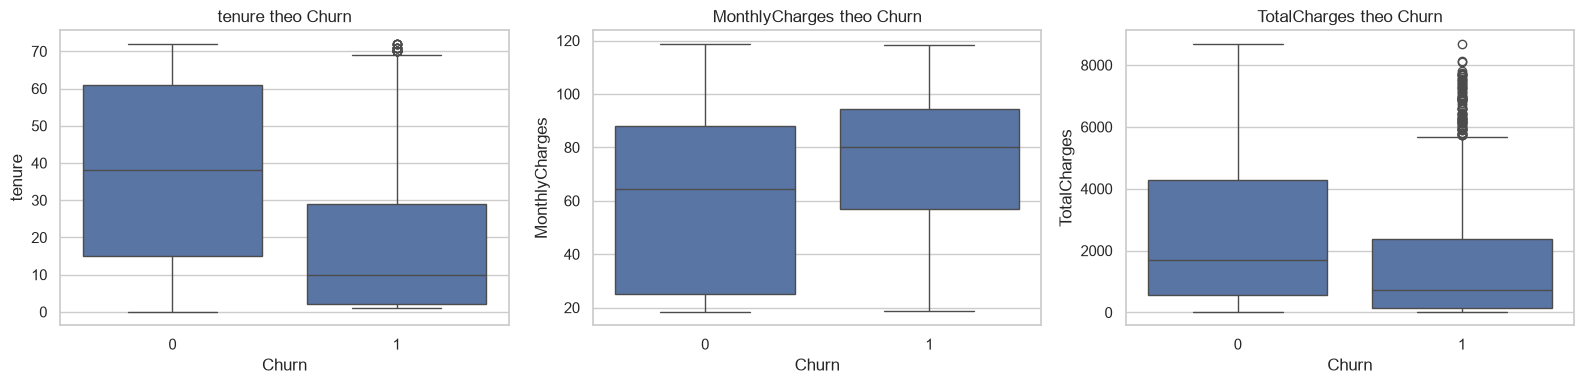
\includegraphics[width=\textwidth]{img/eda_numeric_boxplot.png}
\caption{Phân bố \texttt{tenure}, \texttt{MonthlyCharges}, \texttt{TotalCharges} theo Churn (tập train)}
\end{figure}

\begin{itemize}
    \item Khách hàng rời bỏ có xu hướng có \texttt{tenure} ngắn hơn rõ rệt; hệ số tương quan giữa \texttt{tenure} và Churn khoảng $-0{,}35$.
    \item Nhóm rời bỏ có \texttt{MonthlyCharges} nghiêng về mức cao (tương quan khoảng $+0{,}20$) và \texttt{TotalCharges} thấp hơn (tương quan khoảng $-0{,}19$).
    \item \texttt{tenure} và \texttt{TotalCharges} tương quan cao (khoảng $0{,}83$), \texttt{MonthlyCharges} và \texttt{TotalCharges} tương quan khoảng $0{,}65$. Điều này hợp lý vì tổng chi phí xấp xỉ bằng chi phí tháng nhân thời gian sử dụng.
    \item Một số điểm nằm ngoài râu boxplot nhưng đều nằm trong miền giá trị hợp lý, nên \textbf{không bị loại bỏ}.
\end{itemize}

\begin{figure}[H]
\centering
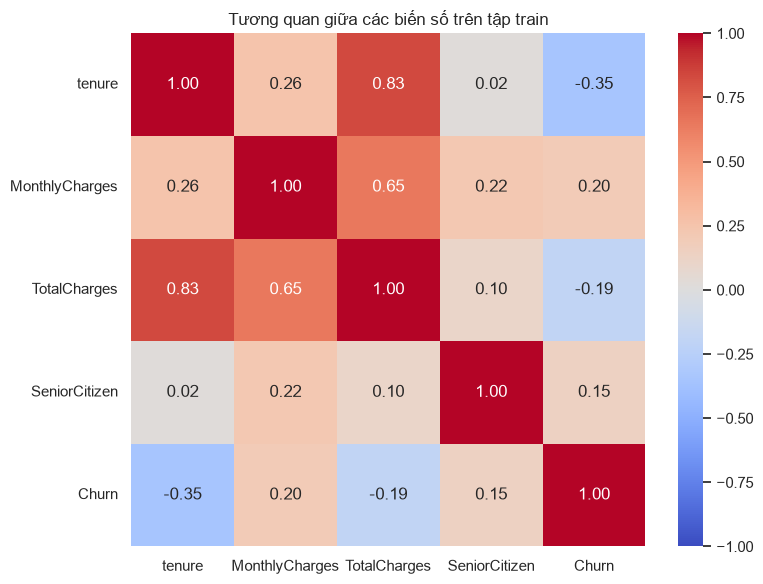
\includegraphics[width=0.55\textwidth]{img/eda_correlation.png}
\caption{Ma trận tương quan giữa các biến số và Churn trên tập train}
\end{figure}

\subsubsection{Đặc trưng phân loại}

\begin{table}[H]
\centering
\begin{tabular}{llrr}
\toprule
\textbf{Đặc trưng} & \textbf{Giá trị} & \textbf{Số khách hàng} & \textbf{Tỉ lệ churn} \\
\midrule
\multirow{3}{*}{Contract} & Month-to-month & 3.102 & \textbf{42,75\%} \\
 & One year & 1.173 & 11,08\% \\
 & Two year & 1.359 & 2,87\% \\
\midrule
\multirow{3}{*}{InternetService} & Fiber optic & 2.483 & \textbf{42,09\%} \\
 & DSL & 1.937 & 18,69\% \\
 & No & 1.214 & 7,25\% \\
\midrule
\multirow{4}{*}{PaymentMethod} & Electronic check & 1.891 & \textbf{45,74\%} \\
 & Mailed check & 1.286 & 19,28\% \\
 & Bank transfer (automatic) & 1.244 & 16,16\% \\
 & Credit card (automatic) & 1.213 & 14,92\% \\
\midrule
\multirow{2}{*}{TechSupport} & No & 2.771 & 41,75\% \\
 & Yes & 1.649 & 15,16\% \\
\midrule
\multirow{2}{*}{OnlineSecurity} & No & 2.797 & 41,94\% \\
 & Yes & 1.623 & 14,42\% \\
\midrule
\multirow{2}{*}{SeniorCitizen} & 1 & 920 & 41,09\% \\
 & 0 & 4.714 & 23,70\% \\
\bottomrule
\end{tabular}
\caption{Tỉ lệ churn theo một số đặc trưng phân loại (tập train)}
\end{table}

\begin{figure}[H]
\centering
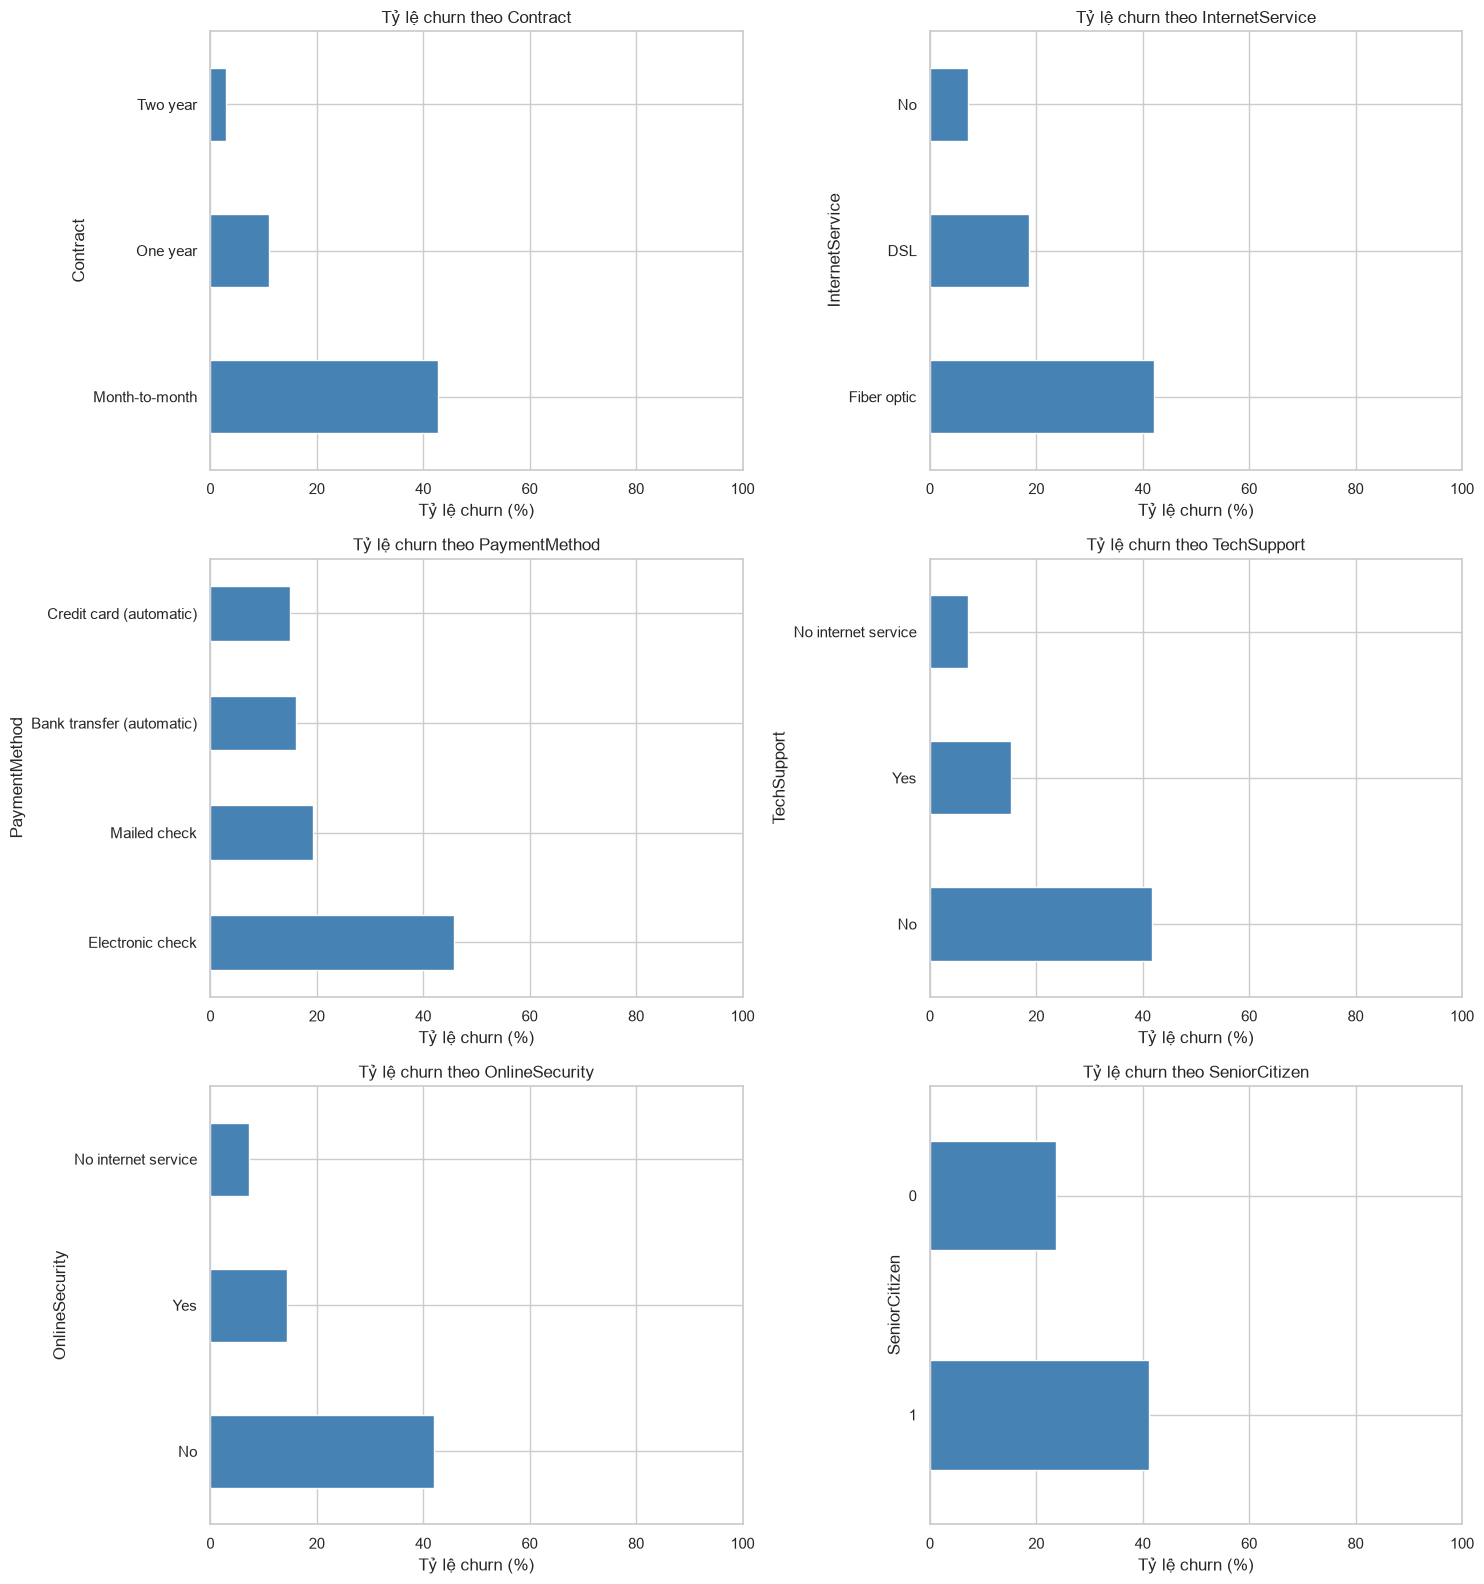
\includegraphics[width=0.85\textwidth]{img/eda_categorical_churn_rate.png}
\caption{Tỉ lệ churn theo các đặc trưng phân loại tiêu biểu}
\end{figure}

Nhận xét chính:
\begin{itemize}
    \item \textbf{Loại hợp đồng} là yếu tố phân tách mạnh nhất: hợp đồng theo tháng có tỉ lệ churn cao gấp gần 15 lần hợp đồng hai năm.
    \item Khách hàng dùng \textbf{Fiber optic}, thanh toán bằng \textbf{Electronic check}, \textbf{không} đăng ký TechSupport/OnlineSecurity hoặc là \textbf{người cao tuổi} có tỉ lệ churn cao hơn hẳn.
    \item Đây là các mối liên hệ quan sát được từ dữ liệu, chưa chứng minh quan hệ nhân quả và chưa xét tương tác giữa các yếu tố (ví dụ Fiber optic thường đi kèm mức phí cao).
\end{itemize}

\subsection{Pipeline tiền xử lý}
Từ kết quả EDA, nhóm xây dựng bộ tiền xử lý bằng \texttt{ColumnTransformer} của \texttt{scikit-learn} (\texttt{src/preprocessing.py}). Đặc trưng được chia thành ba nhóm:

\begin{table}[H]
\centering
\begin{tabular}{p{3.2cm} p{5.5cm} p{6.5cm}}
\toprule
\textbf{Nhóm} & \textbf{Cột} & \textbf{Biến đổi} \\
\midrule
Số (3) & \texttt{tenure}, \texttt{MonthlyCharges}, \texttt{TotalCharges} & \texttt{SimpleImputer(median)} $\rightarrow$ \texttt{StandardScaler} (chỉ với Logistic Regression) \\
Nhị phân (1) & \texttt{SeniorCitizen} & Giữ nguyên mã 0/1 (\texttt{passthrough}) \\
Phân loại (15) & Các cột còn lại & \texttt{SimpleImputer(most\_frequent)} $\rightarrow$ \texttt{OneHotEncoder(handle\_unknown="ignore")} \\
\bottomrule
\end{tabular}
\caption{Các bước tiền xử lý theo nhóm đặc trưng}
\end{table}

\begin{lstlisting}[style=pythonstyle, caption={Hàm xây dựng bộ tiền xử lý trong \texttt{src/preprocessing.py}}]
def build_preprocessor(scale_numeric: bool = True) -> ColumnTransformer:
    numeric_steps = [("imputer", SimpleImputer(strategy="median"))]
    if scale_numeric:
        numeric_steps.append(("scaler", StandardScaler()))

    categorical_pipeline = Pipeline(steps=[
        ("imputer", SimpleImputer(strategy="most_frequent")),
        ("encoder", OneHotEncoder(handle_unknown="ignore",
                                  sparse_output=False)),
    ])
    return ColumnTransformer(
        transformers=[
            ("numeric", Pipeline(numeric_steps), NUMERIC_FEATURES),
            ("binary", "passthrough", BINARY_FEATURES),
            ("categorical", categorical_pipeline, CATEGORICAL_FEATURES),
        ],
        remainder="drop",
    )
\end{lstlisting}

Các quyết định thiết kế:
\begin{itemize}
    \item \texttt{customerID} được giữ lại để truy vết và tái tạo cách chia dữ liệu nhưng bị loại khỏi đầu vào mô hình (\texttt{remainder="drop"}).
    \item Sau One-Hot Encoding, 19 đặc trưng gốc trở thành vector khoảng 45 chiều.
    \item \texttt{handle\_unknown="ignore"} giúp pipeline không bị lỗi khi dự đoán khách hàng mới có giá trị phân loại chưa từng gặp (được kiểm thử trực tiếp trong \texttt{preprocessing.py}).
    \item \texttt{StandardScaler} chỉ được bật cho Logistic Regression (hàm \texttt{requires\_scaling()}), vì các mô hình cây không phụ thuộc vào thang đo.
    \item Bộ tiền xử lý và mô hình được ghép trong một \texttt{Pipeline} duy nhất. Khi cross-validation, imputer/scaler/encoder chỉ được \texttt{fit} trên phần huấn luyện của từng fold, tránh \textbf{rò rỉ dữ liệu} (\textit{data leakage}) từ fold validation.
\end{itemize}

\subsection{Feature Engineering}
Dựa trên các quan sát từ EDA, nhóm xây dựng 9 đặc trưng mới trong transformer \texttt{ChurnFeatureEngineer} (\texttt{src/features.py}):

\begin{table}[H]
\centering
\begin{tabular}{l l p{8.3cm}}
\toprule
\textbf{Loại} & \textbf{Đặc trưng} & \textbf{Cách tính và lý do} \\
\midrule
\multirow{3}{*}{Số} & \texttt{num\_services} & Số dịch vụ khách hàng đăng ký: số cột có giá trị ``Yes'' trong 8 cột dịch vụ, cộng 1 nếu có dùng Internet. Khách dùng nhiều dịch vụ được kỳ vọng gắn bó hơn. \\
 & \texttt{avg\_monthly\_charge} & \texttt{TotalCharges / tenure}; khách có \texttt{tenure} $=0$ (chưa có \texttt{TotalCharges}) lấy \texttt{MonthlyCharges}. \\
 & \texttt{charge\_diff} & \texttt{MonthlyCharges} $-$ \texttt{avg\_monthly\_charge}; dương nghĩa là phí hiện tại cao hơn mức trung bình đã trả (vừa tăng giá hoặc nâng gói). \\
\midrule
\multirow{3}{*}{Nhị phân} & \texttt{is\_new\_month\_to\_month} & 1 nếu hợp đồng theo tháng \textit{và} \texttt{tenure} $\le 12$ -- nhóm rủi ro cao nhất theo EDA. \\
 & \texttt{fiber\_no\_tech\_support} & 1 nếu dùng Fiber optic nhưng không đăng ký TechSupport. \\
 & \texttt{is\_auto\_payment} & 1 nếu thanh toán tự động (chuyển khoản hoặc thẻ tín dụng). \\
\midrule
\multirow{3}{*}{Phân loại} & \texttt{tenure\_group} & Rời rạc hóa \texttt{tenure} thành 0--12, 13--24, 25--48, 49+ tháng. \\
 & \texttt{monthly\_charge\_group} & Chia \texttt{MonthlyCharges} thành 4 nhóm theo tứ phân vị (Q1--Q4). \\
 & \texttt{contract\_tenure} & Kết hợp Contract và \texttt{tenure\_group}, ví dụ ``Month-to-month\_0-12''. \\
\bottomrule
\end{tabular}
\caption{Các đặc trưng mới trong Feature Engineering}
\end{table}

Thiết kế cài đặt:
\begin{itemize}
    \item \texttt{ChurnFeatureEngineer} là một transformer theo chuẩn \texttt{scikit-learn} (\texttt{BaseEstimator}, \texttt{TransformerMixin}), được đặt làm bước đầu tiên của \texttt{Pipeline}, trước \texttt{ColumnTransformer}. Nhờ vậy các đặc trưng được tạo nhất quán cho train, validation, test và khách hàng mới trong \texttt{predict.py}.
    \item Ngưỡng chia nhóm \texttt{MonthlyCharges} là tứ phân vị \textbf{học từ dữ liệu} trong hàm \texttt{fit}. Vì transformer nằm trong Pipeline, các ngưỡng này chỉ được tính trên phần huấn luyện của mỗi fold, không rò rỉ thông tin từ fold validation. Ngưỡng ngoài cùng được đặt là $\pm\infty$ để mọi giá trị mới đều thuộc một nhóm.
    \item Đặc trưng số mới đi qua nhánh imputer/scaler, đặc trưng nhị phân giữ nguyên, đặc trưng phân loại mới đi qua nhánh One-Hot Encoding. Sau FE, dữ liệu có 28 cột trước khi mã hóa.
    \item Bật bằng tham số dòng lệnh \texttt{--feature-engineering} của \texttt{train.py} và \texttt{tune.py}.
\end{itemize}

\begin{lstlisting}[style=pythonstyle, caption={Một phần \texttt{ChurnFeatureEngineer} trong \texttt{src/features.py}}]
def fit(self, X, y=None):
    # Nguong nhom MonthlyCharges hoc tu fold train (tu phan vi).
    quantiles = np.linspace(0, 1, self.n_charge_bins + 1)
    edges = np.quantile(X["MonthlyCharges"], quantiles)
    edges[0], edges[-1] = -np.inf, np.inf
    self.charge_edges_ = np.unique(edges)
    return self

def transform(self, X):
    X = X.copy()
    tenure = X["tenure"]
    X["avg_monthly_charge"] = np.where(
        tenure > 0, X["TotalCharges"] / tenure.where(tenure > 0),
        X["MonthlyCharges"])
    X["charge_diff"] = X["MonthlyCharges"] - X["avg_monthly_charge"]
    X["is_new_month_to_month"] = (
        X["Contract"].eq("Month-to-month") & (tenure <= 12)).astype(int)
    ...
\end{lstlisting}

\section{Mô hình và pipeline huấn luyện}

\subsection{Kiến trúc tổng thể}
Mã nguồn được tổ chức thành các module độc lập trong thư mục \texttt{src/}, mỗi module đảm nhiệm một bước của pipeline:

\begin{table}[H]
\centering
\begin{tabular}{l p{11.5cm}}
\toprule
\textbf{Module} & \textbf{Chức năng} \\
\midrule
\texttt{data.py} & Đọc, kiểm tra và làm sạch dữ liệu; tải lại tập train/test theo danh sách \texttt{customerID} đã lưu. \\
\texttt{features.py} & Transformer \texttt{ChurnFeatureEngineer} tạo 9 đặc trưng mới (Experiment 2). \\
\texttt{preprocessing.py} & Xây dựng \texttt{ColumnTransformer} (imputation, One-Hot Encoding, scaling). \\
\texttt{models.py} & Khởi tạo bốn mô hình (có hoặc không có trọng số lớp) và quy định mô hình nào cần chuẩn hóa. \\
\texttt{train.py} & Chạy Stratified K-Fold Cross-Validation (\texttt{cv}) hoặc huấn luyện trên toàn bộ tập train và lưu pipeline (\texttt{fit}); tùy chọn \texttt{--feature-engineering} và \texttt{--imbalance}. \\
\texttt{compare.py} & So sánh hai lần chạy CV theo từng fold (paired): chênh lệch trung bình và số fold cải thiện. \\
\texttt{tune.py} & Tối ưu siêu tham số bằng \texttt{RandomizedSearchCV} trên đúng 5 fold, lưu pipeline tốt nhất. \\
\texttt{threshold.py} & Chọn ngưỡng quyết định trên xác suất out-of-fold của tập train (tối đa F1 hoặc F2). \\
\texttt{evaluate.py} & Nạp pipeline đã lưu và ngưỡng đã chọn, đánh giá trên tập test, vẽ Confusion Matrix, đường ROC và Precision--Recall. \\
\texttt{predict.py} & Dự đoán xác suất churn cho khách hàng mới từ file CSV. \\
\bottomrule
\end{tabular}
\caption{Các module trong mã nguồn}
\end{table}

\begin{figure}[H]
\centering
\begin{tikzpicture}[
    node distance=0.6cm and 0.5cm,
    box/.style={rectangle, rounded corners, draw=black!70, fill=blue!8, minimum height=1cm, text width=2.3cm, align=center, font=\small},
    arrow/.style={-{Stealth[length=2.5mm]}, thick}
]
\node[box] (raw) {CSV gốc\\(7.043 dòng)};
\node[box, right=of raw] (clean) {Làm sạch\\\texttt{data.py}};
\node[box, right=of clean] (split) {Chia 80/20\\stratified};
\node[box, right=of split] (cv) {5-fold CV\\trên train};
\node[box, below=of cv] (fit) {Fit trên\\toàn bộ train};
\node[box, left=of fit] (test) {Đánh giá\\trên test};
\node[box, left=of test] (pred) {Dự đoán\\khách hàng mới};

\draw[arrow] (raw) -- (clean);
\draw[arrow] (clean) -- (split);
\draw[arrow] (split) -- (cv);
\draw[arrow] (cv) -- node[right, font=\footnotesize]{chọn cấu hình} (fit);
\draw[arrow] (fit) -- (test);
\draw[arrow] (test) -- (pred);
\end{tikzpicture}
\caption{Luồng xử lý của pipeline}
\end{figure}

Mỗi mô hình được đóng gói thành một \texttt{Pipeline} gồm các bước \texttt{features} (chỉ khi bật Feature Engineering), \texttt{preprocessor}, \texttt{smote} (chỉ khi dùng SMOTE) và \texttt{model}:

\begin{lstlisting}[style=pythonstyle, caption={Xây dựng pipeline huấn luyện trong \texttt{src/train.py} (rút gọn)}]
def build_training_pipeline(model_name, feature_engineering=False,
                            imbalance="none", balance_ratio=None):
    steps = []
    if feature_engineering:
        steps.append(("features", ChurnFeatureEngineer()))
    steps.append(("preprocessor", build_preprocessor(
        scale_numeric=requires_scaling(model_name),
        feature_engineering=feature_engineering)))
    if imbalance == "smote":
        steps.append(("smote", SMOTE(random_state=RANDOM_STATE)))
    steps.append(("model", build_model(
        model_name, random_state=RANDOM_STATE,
        balance_ratio=balance_ratio if imbalance == "class_weight" else None)))
    if imbalance == "smote":
        return ImbPipeline(steps=steps)  # chi resample khi fit
    return Pipeline(steps=steps)
\end{lstlisting}

Nhờ vậy, file \texttt{.joblib} được lưu chứa cả bộ tiền xử lý lẫn mô hình; \texttt{evaluate.py} và \texttt{predict.py} chỉ cần nạp lại file này mà không phải tiền xử lý thủ công. Mỗi lần chạy thực nghiệm đều lưu \texttt{config.json} (random state, số fold, danh sách đặc trưng, siêu tham số) cùng kết quả từng fold để có thể tái lập và đối chiếu.

\subsection{Cấu hình các mô hình baseline}
Ở giai đoạn baseline, các mô hình dùng siêu tham số mặc định (hoặc gần mặc định), chưa tinh chỉnh và chưa xử lý mất cân bằng:

\begin{table}[H]
\centering
\begin{tabular}{l p{9.5cm} c}
\toprule
\textbf{Mô hình} & \textbf{Siêu tham số chính} & \textbf{Scaling} \\
\midrule
Logistic Regression & \texttt{solver="lbfgs"}, \texttt{C=1.0}, \texttt{max\_iter=2000} & Có \\
Decision Tree & \texttt{criterion="gini"}, \texttt{max\_depth=None}, \texttt{min\_samples\_split=2} & Không \\
Random Forest & \texttt{n\_estimators=100}, \texttt{max\_features="sqrt"}, \texttt{max\_depth=None} & Không \\
XGBoost & \texttt{n\_estimators=100}, \texttt{learning\_rate=0.1}, \texttt{max\_depth=6}, \texttt{tree\_method="hist"} & Không \\
\bottomrule
\end{tabular}
\caption{Cấu hình baseline (\texttt{random\_state=42} cho mọi mô hình)}
\end{table}

\subsection{Quy trình đánh giá}

\subsubsection{Cross-validation}
Việc so sánh và lựa chọn mô hình được thực hiện bằng \textbf{Stratified 5-Fold Cross-Validation} trên tập train (5.634 khách hàng). Các fold được sinh một lần với \texttt{random\_state=42} và dùng chung cho mọi mô hình, nên kết quả giữa các mô hình và giữa các lần chạy có thể so sánh trực tiếp. Kết quả được báo cáo dưới dạng \textit{trung bình $\pm$ độ lệch chuẩn} qua 5 fold; độ lệch chuẩn mô tả mức dao động giữa các fold, không phải khoảng tin cậy.

Ngoài điểm validation, nhóm ghi lại điểm trên phần huấn luyện của từng fold (\texttt{return\_train\_score=True}) để đo \textbf{khoảng cách train--validation}, dùng làm dấu hiệu nhận biết overfitting.

\subsubsection{Đánh giá cuối trên tập test}
Sau khi chọn cấu hình bằng cross-validation, quy trình cuối gồm ba lệnh:
\begin{enumerate}
    \item \texttt{python -m src.tune --fit}: tìm siêu tham số và lưu pipeline tốt nhất (đã huấn luyện lại trên toàn bộ tập train) vào \texttt{outputs/models/tuned/}.
    \item \texttt{python -m src.threshold}: chọn ngưỡng quyết định trên xác suất out-of-fold của tập train, ghi vào \texttt{thresholds.json}.
    \item \texttt{python -m src.evaluate --model-dir outputs/models/tuned}: đánh giá một lần duy nhất trên tập test 1.409 khách hàng với ngưỡng đã chọn.
\end{enumerate}
Mọi lựa chọn (cấu hình, siêu tham số, ngưỡng, mô hình cuối) đều được quyết định trước khi dùng tập test.

\subsubsection{Các chỉ số đánh giá}
Với lớp dương là ``rời bỏ'' (Churn $=1$), gọi TP, FP, TN, FN là các ô của Confusion Matrix:
\begin{align}
    \text{Accuracy}  &= \frac{TP + TN}{TP + TN + FP + FN} \\
    \text{Precision} &= \frac{TP}{TP + FP} \qquad
    \text{Recall} = \frac{TP}{TP + FN} \\
    \text{F1}        &= 2 \cdot \frac{\text{Precision} \cdot \text{Recall}}{\text{Precision} + \text{Recall}}
\end{align}
\begin{itemize}
    \item \textbf{Precision}: trong số khách hàng bị dự đoán rời bỏ, bao nhiêu phần trăm thực sự rời bỏ -- liên quan đến chi phí lãng phí ưu đãi.
    \item \textbf{Recall}: trong số khách hàng thực sự rời bỏ, mô hình phát hiện được bao nhiêu -- liên quan đến doanh thu bị mất do bỏ sót.
    \item \textbf{F1-score}: trung bình điều hòa của Precision và Recall, là chỉ số chính để so sánh trên dữ liệu mất cân bằng.
    \item \textbf{ROC-AUC}: diện tích dưới đường ROC, đo khả năng \textit{xếp hạng} khách hàng theo rủi ro, không phụ thuộc vào ngưỡng phân loại.
    \item \textbf{PR-AUC} (\textit{average precision}): diện tích dưới đường Precision--Recall. Cũng không phụ thuộc ngưỡng nhưng tập trung vào lớp thiểu số, nên nhạy hơn ROC-AUC khi dữ liệu mất cân bằng. Mức ngẫu nhiên của PR-AUC bằng tỉ lệ lớp dương (khoảng 0,265), trong khi của ROC-AUC là 0,5. PR-AUC là chỉ số dùng để chọn siêu tham số và mô hình cuối cùng.
\end{itemize}

\section{Thực nghiệm và đánh giá}

Các thực nghiệm được thiết kế để trả lời từng câu hỏi riêng biệt. Mọi thực nghiệm dùng cùng tập train/test, cùng 5 fold Stratified và cùng tập chỉ số, chỉ thay đổi một yếu tố tại một thời điểm.

\begin{table}[H]
\centering
\begin{tabular}{c p{6cm} p{6.5cm}}
\toprule
\textbf{Thực nghiệm} & \textbf{Câu hỏi} & \textbf{Cách đánh giá} \\
\midrule
1 & So sánh 4 thuật toán ở cấu hình baseline & 5-fold CV \\
2 & Feature Engineering có cải thiện hiệu năng? & 5-fold CV, so sánh cặp theo fold \\
3 & Class weight hay SMOTE giải quyết mất cân bằng tốt hơn? & 5-fold CV, so sánh cặp theo fold \\
4 & Hyperparameter Tuning cải thiện bao nhiêu? & RandomizedSearchCV trên cùng 5 fold \\
5 & Ngưỡng quyết định nào phù hợp? & Xác suất out-of-fold trên tập train \\
-- & Mô hình cuối cùng và giải thích mô hình & Tập test (dùng một lần) \\
\bottomrule
\end{tabular}
\caption{Tổng quan các thực nghiệm}
\end{table}

So với kế hoạch ban đầu, nhóm không thực hiện thực nghiệm so sánh các phương pháp Encoding/Scaling; mọi thực nghiệm dùng chung One-Hot Encoding và \texttt{StandardScaler} (chỉ cho Logistic Regression).

% ============================================================
\subsection{Experiment 1: So sánh các mô hình baseline}
% ============================================================

\subsubsection{Kết quả cross-validation}

\begin{table}[H]
\centering
\small
\begin{tabular}{lccccc}
\toprule
\textbf{Mô hình} & \textbf{Accuracy} & \textbf{Precision} & \textbf{Recall} & \textbf{F1} & \textbf{ROC-AUC} \\
\midrule
Logistic Regression & \textbf{0,8019} $\pm$ 0,0133 & \textbf{0,6524} $\pm$ 0,0294 & \textbf{0,5431} $\pm$ 0,0460 & \textbf{0,5921} $\pm$ 0,0334 & \textbf{0,8461} $\pm$ 0,0140 \\
XGBoost             & 0,7982 $\pm$ 0,0088 & 0,6501 $\pm$ 0,0255 & 0,5204 $\pm$ 0,0235 & 0,5777 $\pm$ 0,0183 & 0,8413 $\pm$ 0,0084 \\
Random Forest       & 0,7863 $\pm$ 0,0092 & 0,6276 $\pm$ 0,0261 & 0,4803 $\pm$ 0,0215 & 0,5439 $\pm$ 0,0193 & 0,8199 $\pm$ 0,0114 \\
Decision Tree       & 0,7286 $\pm$ 0,0060 & 0,4890 $\pm$ 0,0108 & 0,4957 $\pm$ 0,0141 & 0,4922 $\pm$ 0,0082 & 0,6543 $\pm$ 0,0057 \\
\bottomrule
\end{tabular}
\caption{Kết quả validation của 4 mô hình baseline (Stratified 5-fold CV trên tập train, 19 đặc trưng gốc)}
\label{tab:baseline_cv}
\end{table}

\begin{figure}[H]
\centering
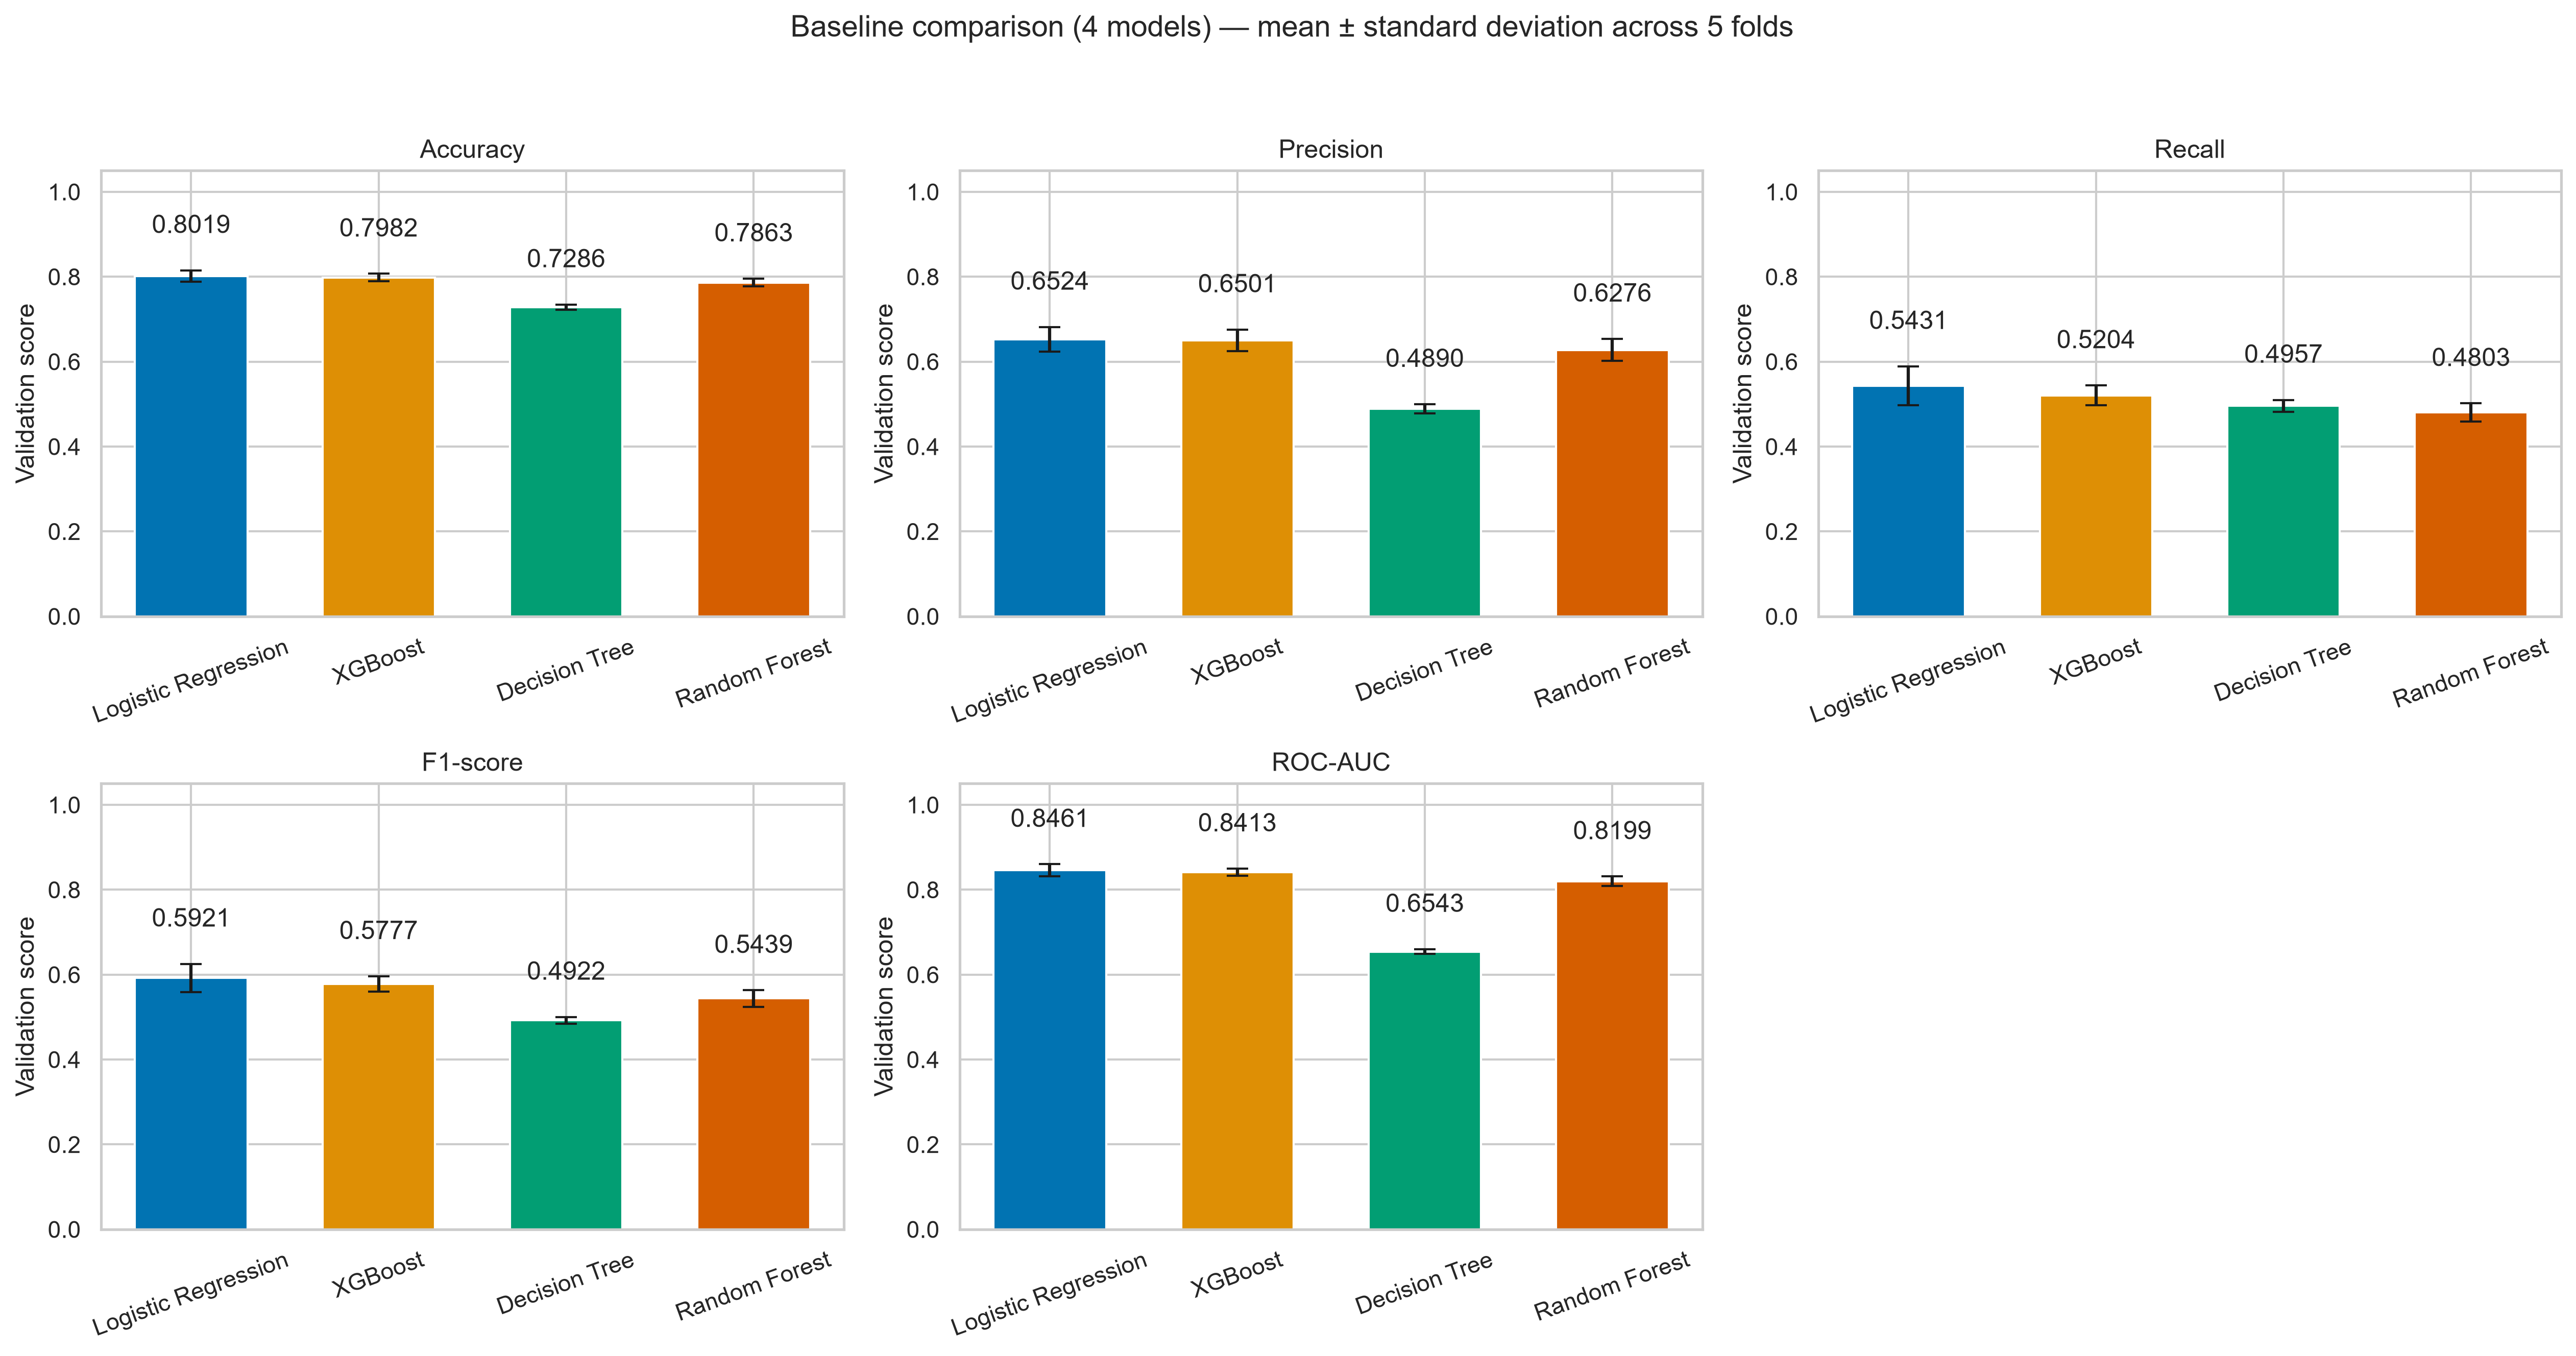
\includegraphics[width=\textwidth]{img/baseline_validation_all_models.png}
\caption{So sánh các chỉ số validation của 4 mô hình baseline (thanh lỗi: độ lệch chuẩn qua 5 fold)}
\end{figure}

Nhận xét:
\begin{itemize}
    \item Theo F1 và ROC-AUC, thứ tự các mô hình là: \textbf{Logistic Regression $>$ XGBoost $>$ Random Forest $>$ Decision Tree}. Ở cấu hình mặc định, các mô hình dựa trên cây chưa vượt được mô hình tuyến tính.
    \item Logistic Regression và XGBoost rất gần nhau (chênh lệch F1 khoảng 0,014 và ROC-AUC khoảng 0,005, nhỏ hơn độ lệch chuẩn giữa các fold), nên chưa thể kết luận mô hình nào tốt hơn.
    \item Random Forest thấp hơn Logistic Regression khoảng 0,05 ở F1 và 0,026 ở ROC-AUC. Decision Tree thấp hơn hẳn, đặc biệt ROC-AUC chỉ 0,654 do cây không giới hạn độ sâu cho xác suất gần như chỉ nhận giá trị 0 hoặc 1.
    \item \textbf{Recall của cả bốn mô hình chỉ khoảng 0,48--0,54}: với ngưỡng mặc định 0,5, mô hình mới phát hiện được khoảng một nửa số khách hàng thực sự rời bỏ. Đây là điểm yếu chung cần cải thiện ở các thực nghiệm sau.
\end{itemize}

\subsubsection{Phân tích overfitting}

\begin{table}[H]
\centering
\begin{tabular}{lcccccc}
\toprule
\textbf{Mô hình} & \textbf{F1 train} & \textbf{F1 val} & \textbf{F1 gap} & \textbf{AUC train} & \textbf{AUC val} & \textbf{AUC gap} \\
\midrule
Logistic Regression & 0,6018 & 0,5921 & 0,0096 & 0,8496 & 0,8461 & 0,0035 \\
XGBoost             & 0,7602 & 0,5777 & 0,1825 & 0,9504 & 0,8413 & 0,1091 \\
Random Forest       & 0,9968 & 0,5439 & 0,4529 & 0,9999 & 0,8199 & 0,1801 \\
Decision Tree       & 0,9968 & 0,4922 & 0,5046 & 1,0000 & 0,6543 & 0,3457 \\
\bottomrule
\end{tabular}
\caption{Khoảng cách giữa điểm train và validation (trung bình 5 fold)}
\end{table}

\begin{figure}[H]
\centering
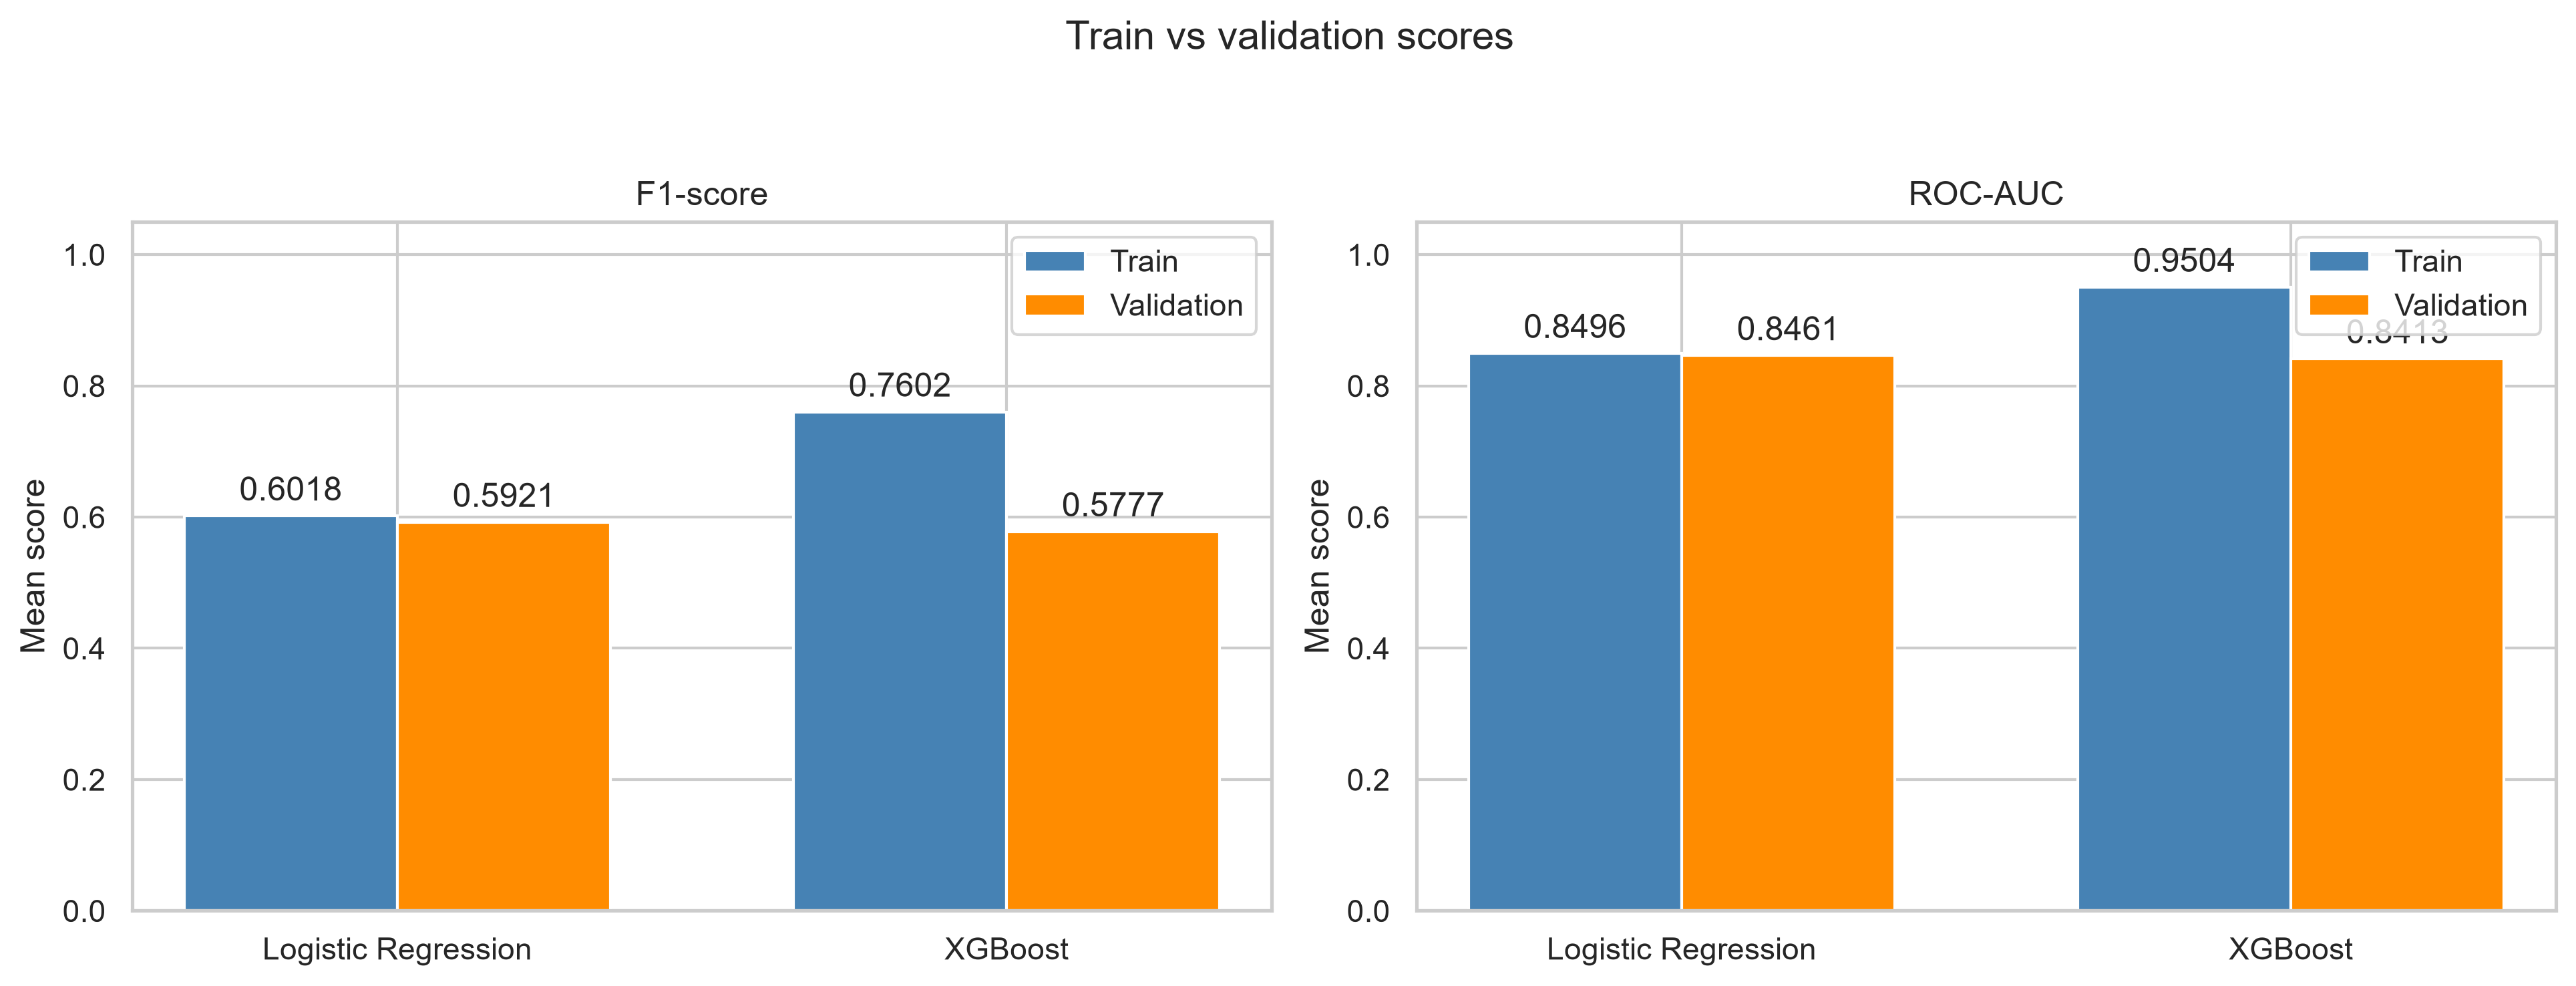
\includegraphics[width=0.49\textwidth]{img/train_vs_val_lr_xgb.png}
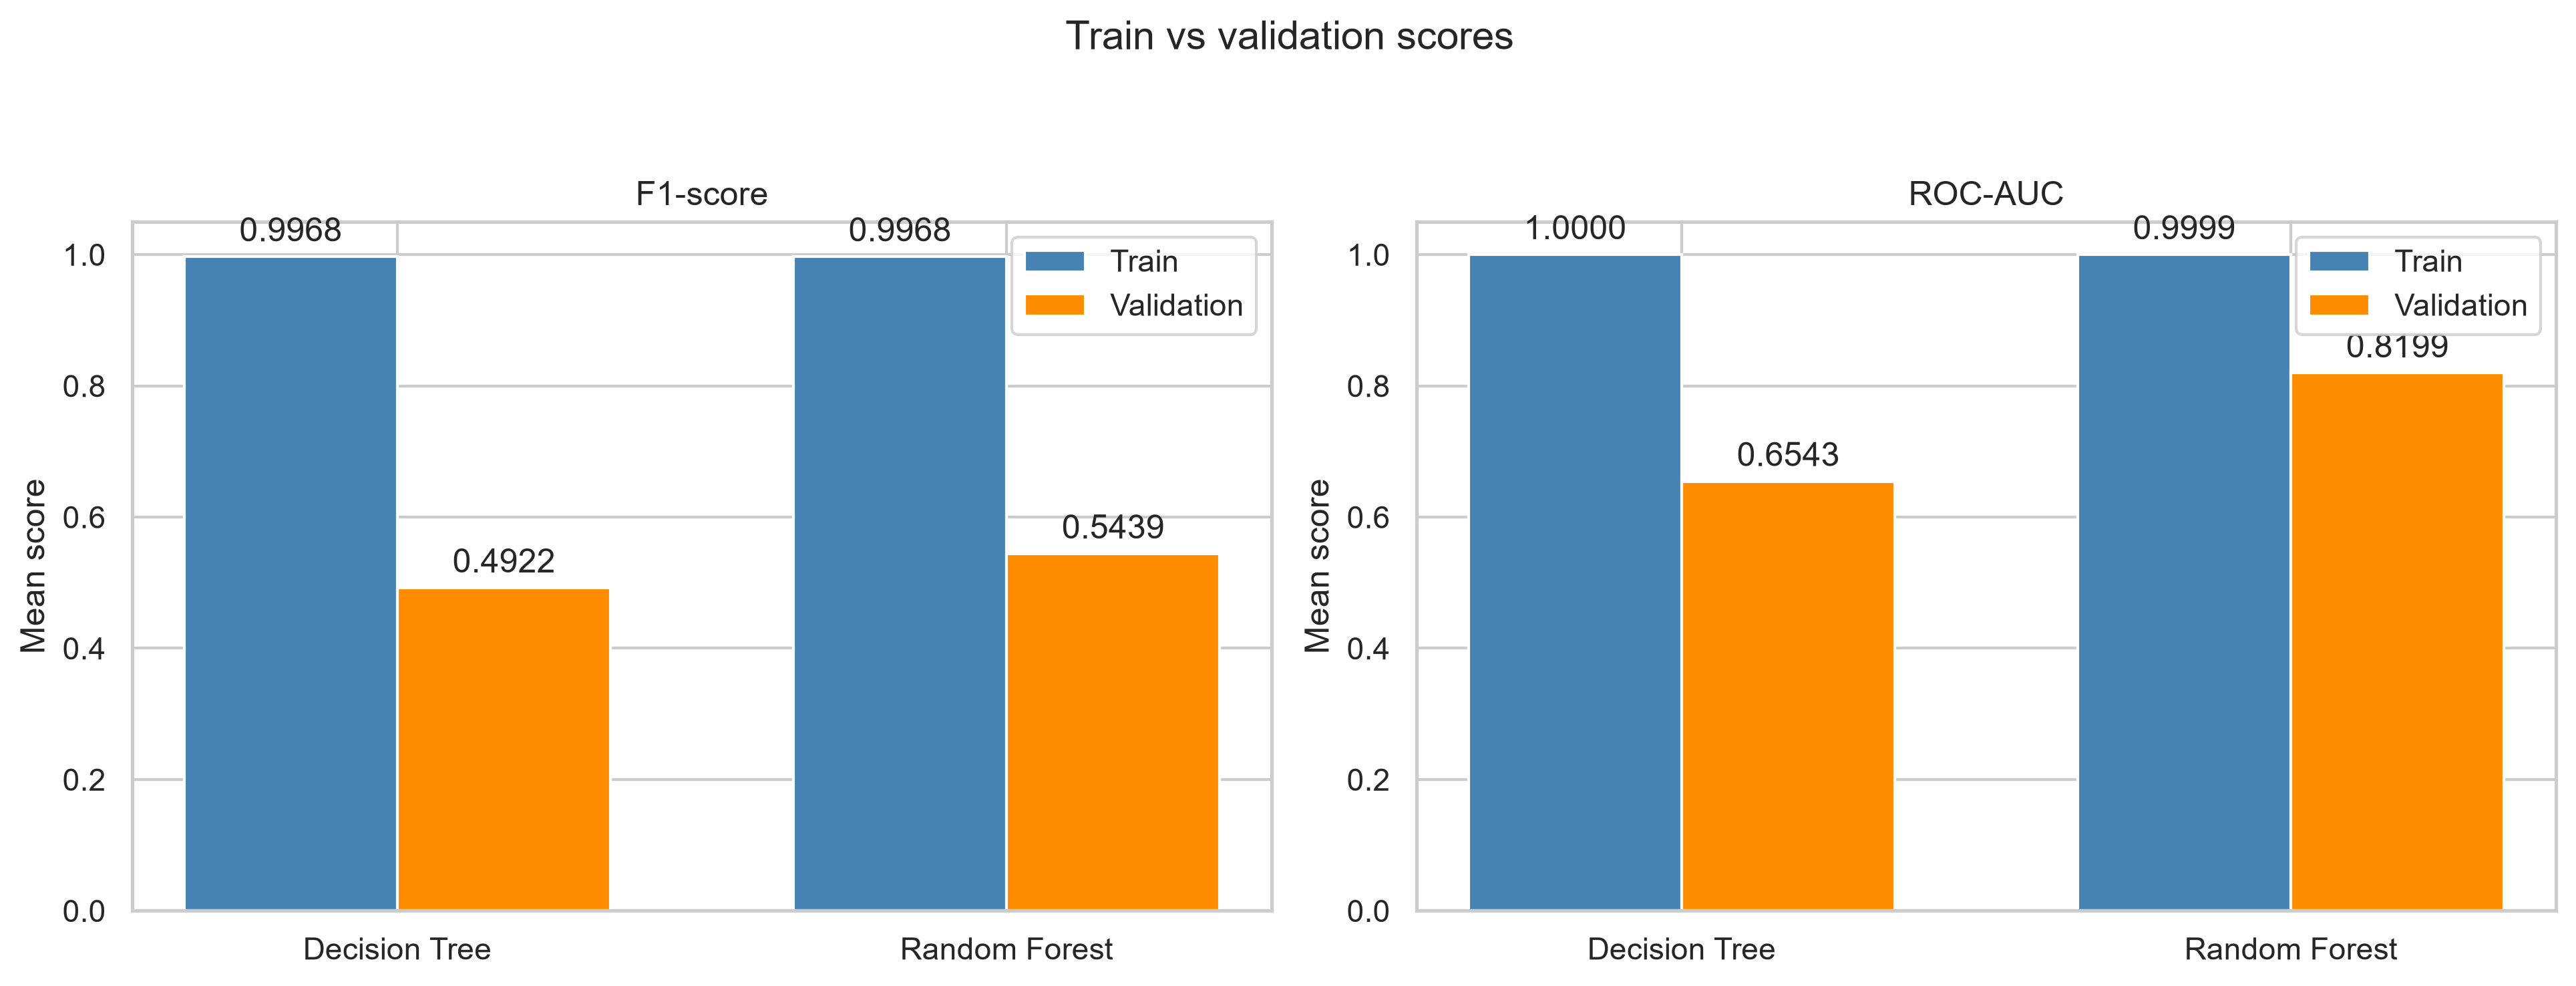
\includegraphics[width=0.49\textwidth]{img/train_vs_val_dt_rf.png}
\caption{F1 và ROC-AUC trên train và validation: Logistic Regression, XGBoost (trái); Decision Tree, Random Forest (phải)}
\end{figure}

\begin{itemize}
    \item \textbf{Logistic Regression} có điểm train và validation gần như trùng nhau: mô hình không overfit, nhưng điểm train thấp cho thấy mô hình tuyến tính có thể đang bị giới hạn về khả năng biểu diễn (\textit{underfit} nhẹ).
    \item \textbf{Decision Tree} và \textbf{Random Forest} gần như ghi nhớ hoàn toàn tập huấn luyện (F1 train $\approx 0{,}997$) do cây phát triển không giới hạn đến khi mỗi lá gần như thuần nhất. Random Forest giảm phương sai nhờ lấy trung bình nhiều cây (ROC-AUC validation tăng từ 0,654 lên 0,820) nhưng từng cây thành phần vẫn overfit.
    \item \textbf{XGBoost} cũng có dấu hiệu overfitting (F1 gap 0,18) ở cấu hình \texttt{max\_depth=6}, 100 cây.
    \item Kết luận: các mô hình cây có nhiều dư địa cải thiện nhất thông qua việc \textbf{giới hạn độ phức tạp} (\texttt{max\_depth}, \texttt{min\_samples\_leaf}, \texttt{min\_samples\_split}) và chính quy hóa -- là trọng tâm của Experiment 4.
\end{itemize}

\subsubsection{Độ ổn định qua các fold}

\begin{figure}[H]
\centering
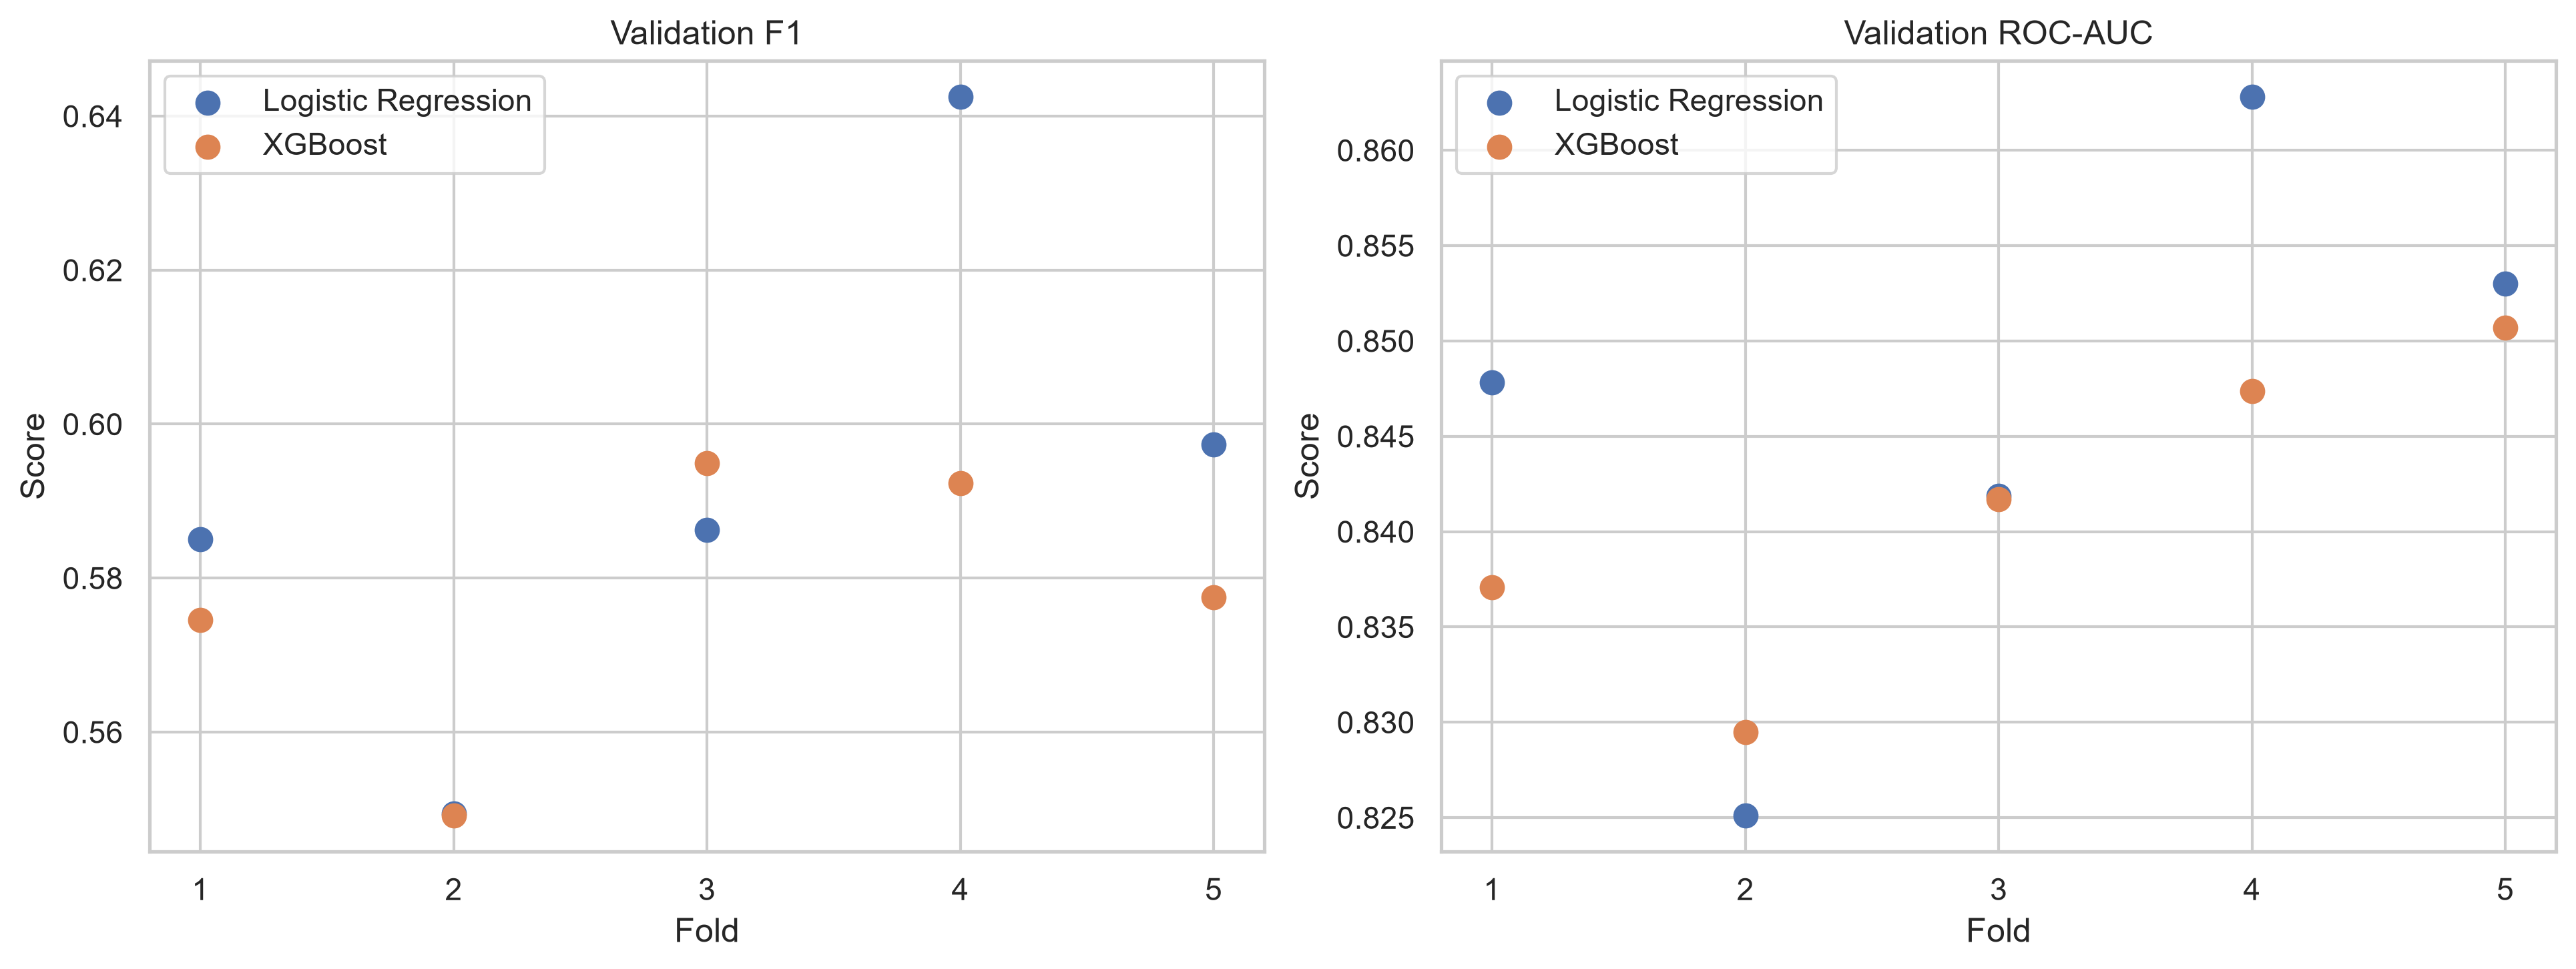
\includegraphics[width=0.49\textwidth]{img/folds_lr_xgb.png}
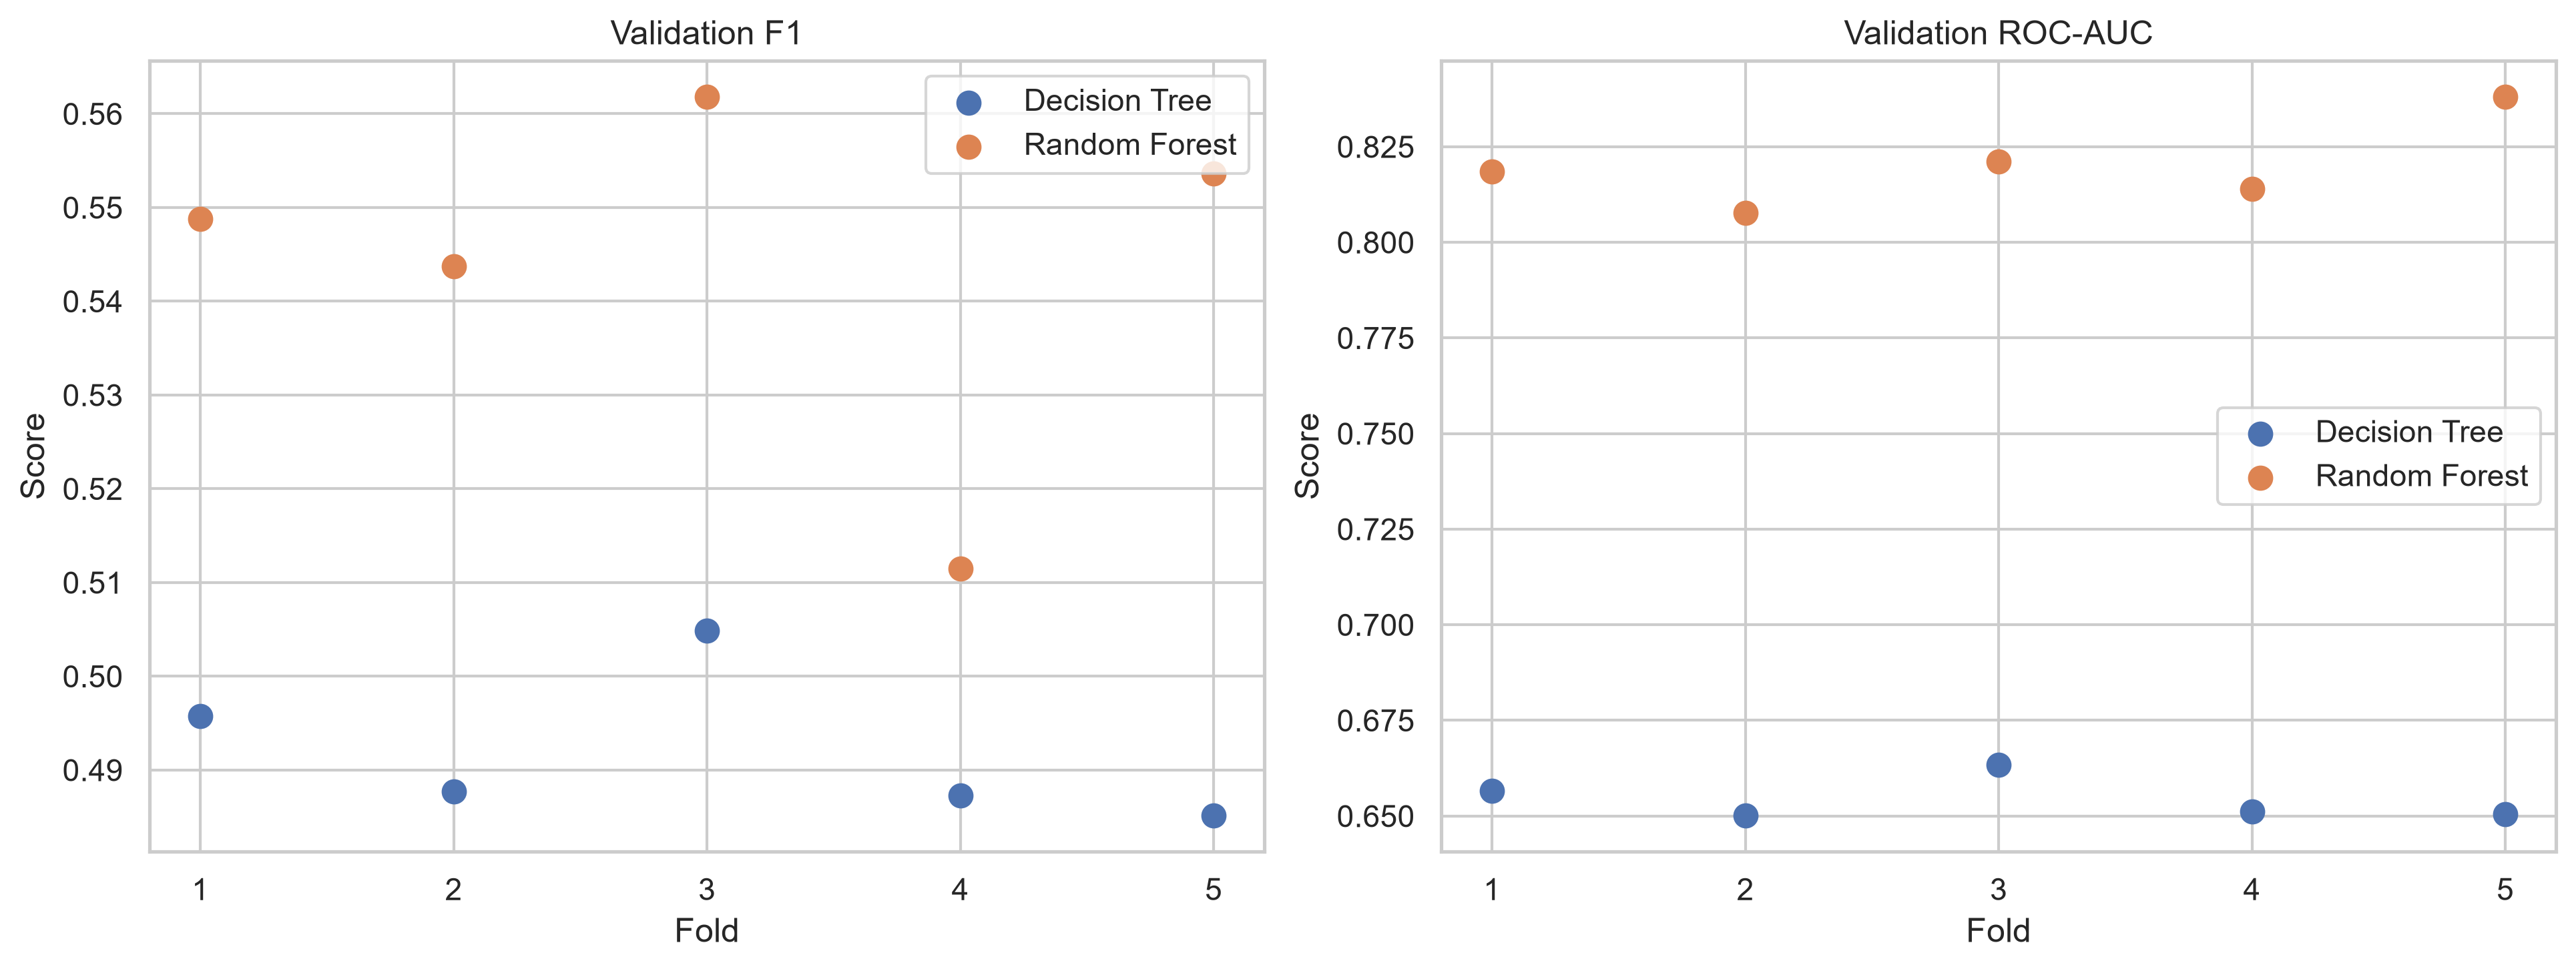
\includegraphics[width=0.49\textwidth]{img/folds_dt_rf.png}
\caption{F1 và ROC-AUC validation trên từng fold}
\end{figure}

Thứ hạng các mô hình tương đối nhất quán qua các fold: Random Forest luôn có ROC-AUC cao hơn Decision Tree ở cả 5 fold (0,808--0,838 so với 0,650--0,663). Logistic Regression có mức dao động F1 lớn nhất (0,550--0,643), trong khi XGBoost ổn định hơn nhưng có điểm trung bình thấp hơn một chút.

\subsubsection{PR-AUC của các mô hình baseline}
Với dữ liệu mất cân bằng, nhóm ghi thêm PR-AUC cho mọi lần chạy. Ở cấu hình baseline, PR-AUC của Logistic Regression là 0,662, XGBoost 0,653, Random Forest 0,610 và Decision Tree chỉ 0,377 (mức ngẫu nhiên khoảng 0,265). Thứ hạng giống với F1 và ROC-AUC.

% ============================================================
\subsection{Experiment 2: Ảnh hưởng của Feature Engineering}
% ============================================================
\textbf{Thiết kế:} thêm bước \texttt{ChurnFeatureEngineer} (9 đặc trưng mới, Mục 3) vào đầu pipeline, giữ nguyên mọi thứ khác (\texttt{python -m src.train cv --feature-engineering}). Để kiểm tra FE có giúp ích khi đã xử lý mất cân bằng hay không, nhóm chạy FE trong cả ba bối cảnh: không xử lý, class weight và SMOTE. Mỗi so sánh được thực hiện \textbf{theo cặp trên từng fold} (\texttt{src/compare.py}): vì mọi lần chạy dùng cùng 5 fold, chênh lệch được tính trên từng fold rồi lấy trung bình, kèm số fold mà cấu hình có FE tốt hơn.

\begin{table}[H]
\centering
\small
\begin{tabular}{lcccccc}
\toprule
\multirow{2}{*}{\textbf{Mô hình}} & \multicolumn{2}{c}{\textbf{Không xử lý}} & \multicolumn{2}{c}{\textbf{Class weight}} & \multicolumn{2}{c}{\textbf{SMOTE}} \\
\cmidrule(lr){2-3} \cmidrule(lr){4-5} \cmidrule(lr){6-7}
 & $\Delta$F1 & $\Delta$PR-AUC & $\Delta$F1 & $\Delta$PR-AUC & $\Delta$F1 & $\Delta$PR-AUC \\
\midrule
Logistic Regression & +0,003 (3/5) & +0,001 (3/5) & +0,001 (2/5) & +0,001 (3/5) & +0,000 (2/5) & $-$0,000 (2/5) \\
Decision Tree & +0,003 (3/5) & +0,003 (3/5) & $-$0,009 (1/5) & $-$0,008 (2/5) & +0,005 (3/5) & +0,003 (3/5) \\
Random Forest & $-$0,010 (2/5) & +0,008 (3/5) & $-$0,005 (1/5) & +0,007 (4/5) & +0,010 (3/5) & +0,007 (4/5) \\
XGBoost & $-$0,012 (1/5) & $-$0,007 (1/5) & $-$0,004 (3/5) & $-$0,003 (3/5) & $-$0,010 (1/5) & $-$0,006 (1/5) \\
\bottomrule
\end{tabular}
\caption{Chênh lệch khi thêm Feature Engineering (trung bình 5 fold; trong ngoặc: số fold cải thiện)}
\label{tab:fe}
\end{table}

\subsubsection{Phân tích}
\begin{itemize}
    \item \textbf{Feature Engineering không mang lại cải thiện đáng kể.} Mọi chênh lệch đều nằm trong khoảng $\pm 0{,}012$, nhỏ hơn độ lệch chuẩn của F1 giữa các fold (0,02--0,03), và không có cấu hình nào cải thiện ở cả 5 fold. Kết quả nhất quán trong cả ba bối cảnh xử lý mất cân bằng.
    \item \textbf{XGBoost giảm nhẹ trong cả ba bối cảnh} (F1 giảm 0,004--0,012, chỉ cải thiện ở 1--3/5 fold). Ở cấu hình mặc định (\texttt{max\_depth=6}), XGBoost đã overfit (Mục 5.1); thêm các đặc trưng liên tục như \texttt{avg\_monthly\_charge}, \texttt{charge\_diff} tạo thêm điểm chia để mô hình khớp nhiễu. F1 train của XGBoost tăng từ 0,760 lên 0,790 trong khi F1 validation giảm.
    \item \textbf{Random Forest tăng nhẹ PR-AUC} (+0,007 đến +0,008, cải thiện ở 3--4/5 fold) nhưng F1 lúc tăng lúc giảm, nên không đủ cơ sở kết luận.
    \item \textbf{Nguyên nhân:} các đặc trưng mới đều được dựng từ thông tin mô hình đã có. Mô hình cây tự học được các ngưỡng (ví dụ \texttt{tenure} $\le 12$) và tương tác (hợp đồng $\times$ thời gian sử dụng), còn Logistic Regression đã nắm được xu hướng chính qua \texttt{tenure}, \texttt{Contract} và \texttt{InternetService}.
    \item \textbf{Kết luận:} FE không được đưa vào cấu hình cuối cùng; các thực nghiệm sau dùng 19 đặc trưng gốc.
\end{itemize}

% ============================================================
\subsection{Experiment 3: Xử lý mất cân bằng dữ liệu}
% ============================================================
\textbf{Thiết kế:} giữ nguyên 19 đặc trưng gốc và siêu tham số baseline, chỉ thay đổi cách xử lý mất cân bằng (\texttt{--imbalance}):
\begin{itemize}
    \item \textbf{Class weight:} \texttt{class\_weight="balanced"} cho Logistic Regression, Decision Tree, Random Forest; với XGBoost dùng \texttt{scale\_pos\_weight} bằng tỉ lệ số mẫu không rời bỏ / rời bỏ ($4.139 / 1.495 \approx 2{,}77$). Cả hai cách đều làm tổng trọng số của hai lớp bằng nhau.
    \item \textbf{SMOTE:} chèn bước \texttt{SMOTE} sau \texttt{preprocessor} trong \texttt{imblearn.pipeline.Pipeline}. Pipeline của \texttt{imblearn} chỉ sinh mẫu khi \texttt{fit}, nên SMOTE chỉ tác động lên phần huấn luyện của mỗi fold; fold validation và tập test giữ nguyên phân bố thật.
\end{itemize}

\begin{table}[H]
\centering
\small
\begin{tabular}{llccccc}
\toprule
\textbf{Mô hình} & \textbf{Chiến lược} & \textbf{Precision} & \textbf{Recall} & \textbf{F1} & \textbf{$\Delta$F1 (fold)} & \textbf{PR-AUC} \\
\midrule
\multirow{3}{*}{Logistic Regression} & Không xử lý & 0,652 & 0,543 & 0,592 & -- & 0,662 \\
 & Class weight & 0,517 & \textbf{0,801} & 0,628 & +0,036 (5/5) & 0,660 \\
 & SMOTE & 0,526 & 0,789 & \textbf{0,631} & +0,039 (5/5) & 0,658 \\
\midrule
\multirow{3}{*}{Decision Tree} & Không xử lý & 0,489 & 0,496 & 0,492 & -- & 0,377 \\
 & Class weight & 0,512 & 0,496 & \textbf{0,504} & +0,012 (4/5) & 0,389 \\
 & SMOTE & 0,479 & 0,495 & 0,487 & $-$0,006 (1/5) & 0,372 \\
\midrule
\multirow{3}{*}{Random Forest} & Không xử lý & 0,628 & 0,480 & 0,544 & -- & 0,610 \\
 & Class weight & 0,563 & \textbf{0,638} & \textbf{0,598} & +0,054 (5/5) & 0,604 \\
 & SMOTE & 0,608 & 0,496 & 0,546 & +0,002 (3/5) & 0,593 \\
\midrule
\multirow{3}{*}{XGBoost} & Không xử lý & 0,650 & 0,520 & 0,578 & -- & 0,653 \\
 & Class weight & 0,545 & \textbf{0,747} & \textbf{0,630} & +0,053 (5/5) & 0,653 \\
 & SMOTE & 0,636 & 0,565 & 0,598 & +0,020 (5/5) & 0,651 \\
\bottomrule
\end{tabular}
\caption{Kết quả validation (5-fold CV, ngưỡng 0,5) của các chiến lược xử lý mất cân bằng}
\label{tab:imbalance}
\end{table}

\subsubsection{Phân tích}
\begin{itemize}
    \item \textbf{Class weight là chiến lược tốt và ổn định nhất.} F1 tăng 0,036--0,054 và tăng ở cả 5/5 fold với Logistic Regression, Random Forest và XGBoost. Recall tăng mạnh: Logistic Regression từ 0,543 lên 0,801, XGBoost từ 0,520 lên 0,747. Mô hình giờ phát hiện được khoảng 3/4 khách hàng rời bỏ thay vì một nửa.
    \item \textbf{Cái giá là Precision giảm} (Logistic Regression: 0,652 xuống 0,517; XGBoost: 0,650 xuống 0,545): mô hình chấp nhận cảnh báo nhầm nhiều hơn để bắt được nhiều khách hàng rời bỏ hơn. Vì Recall tăng nhiều hơn Precision giảm, F1 vẫn tăng. Với bài toán giữ chân khách hàng, bỏ sót một khách hàng sắp rời bỏ thường tốn kém hơn gửi nhầm một ưu đãi, nên đánh đổi này là hợp lý.
    \item \textbf{PR-AUC gần như không đổi} ($|\Delta| \le 0{,}006$ với LR, RF, XGBoost). Class weight không làm mô hình \textit{xếp hạng} khách hàng tốt hơn mà chủ yếu \textit{dịch chuyển xác suất dự đoán} lên cao, tương đương với hạ ngưỡng quyết định.
    \item \textbf{SMOTE hiệu quả với Logistic Regression} (+0,039 F1, tương đương class weight) nhưng yếu hơn với mô hình cây: XGBoost chỉ +0,020, Random Forest gần như không đổi. SMOTE nội suy tuyến tính giữa các mẫu sau One-Hot Encoding nên tạo ra các giá trị không có thật (ví dụ 0,4 cho cột \texttt{Contract\_Two year}); mô hình cây chia theo ngưỡng nên dễ bị ảnh hưởng bởi các mẫu giả này. Class weight đơn giản hơn và không sinh dữ liệu giả.
    \item \textbf{Decision Tree gần như không phản ứng} (Recall vẫn 0,496), và Recall của Random Forest chỉ tăng lên 0,638. Ở cấu hình mặc định, cây phát triển đến khi lá thuần nhất (F1 train $\approx 0{,}997$), nên xác suất dự đoán gần như chỉ là 0 hoặc 1; trọng số lớp không còn tác dụng khi mọi lá đã thuần nhất. Điều này chỉ thay đổi sau khi giới hạn độ phức tạp ở Experiment 4.
    \item \textbf{Kết luận:} chọn \textbf{class weight} cho mọi mô hình ở các bước tiếp theo.
\end{itemize}

% ============================================================
\subsection{Experiment 4: Hyperparameter Tuning}
% ============================================================
\textbf{Thiết kế:} tối ưu siêu tham số bằng \texttt{RandomizedSearchCV} (\texttt{python -m src.tune}) trên cấu hình class weight, 19 đặc trưng gốc. Tìm kiếm dùng đúng 5 fold của các thực nghiệm trước, nên kết quả so sánh cặp được với Experiment 3. Tiêu chí chọn là \textbf{PR-AUC} vì chỉ số này không phụ thuộc ngưỡng và tập trung vào lớp rời bỏ; ngưỡng được chọn riêng ở Experiment 5.

\begin{table}[H]
\centering
\small
\begin{tabular}{l c p{9.8cm}}
\toprule
\textbf{Mô hình} & \textbf{Số tổ hợp} & \textbf{Không gian tìm kiếm} \\
\midrule
Logistic Regression & 30 & \texttt{C} $\sim$ log-uniform$(10^{-3}, 10^{2})$ \\
Decision Tree & 50 & \texttt{max\_depth} $\in [2, 15]$, \texttt{min\_samples\_leaf} $\in [1, 59]$, \texttt{criterion} $\in$ \{gini, entropy\} \\
Random Forest & 40 & \texttt{n\_estimators} $\in [200, 600]$, \texttt{max\_depth} $\in$ \{4, 6, 8, 10, 12, 16, None\}, \texttt{min\_samples\_leaf} $\in [1, 29]$, \texttt{max\_features} $\in$ \{sqrt, log2, 0,5\} \\
XGBoost & 60 & \texttt{n\_estimators} $\in [100, 600]$, \texttt{learning\_rate} $\sim$ log-uniform$(0{,}01; 0{,}3)$, \texttt{max\_depth} $\in [2, 7]$, \texttt{min\_child\_weight} $\in [1, 10]$, \texttt{subsample}, \texttt{colsample\_bytree} $\in [0{,}6; 1]$, \texttt{reg\_lambda} $\sim$ log-uniform$(0{,}1; 10)$ \\
\bottomrule
\end{tabular}
\caption{Không gian tìm kiếm siêu tham số}
\end{table}

\begin{table}[H]
\centering
\small
\begin{tabular}{l p{10cm}}
\toprule
\textbf{Mô hình} & \textbf{Siêu tham số tốt nhất} \\
\midrule
Logistic Regression & \texttt{C=0,92} \\
Decision Tree & \texttt{criterion=entropy}, \texttt{max\_depth=12}, \texttt{min\_samples\_leaf=51} \\
Random Forest & 287 cây, \texttt{max\_depth=8}, \texttt{max\_features=0,5}, \texttt{min\_samples\_leaf=11} \\
XGBoost & 271 cây, \texttt{max\_depth=3}, \texttt{learning\_rate=0,023}, \texttt{min\_child\_weight=5}, \texttt{subsample=0,82}, \texttt{colsample\_bytree=0,96}, \texttt{reg\_lambda=0,79} \\
\bottomrule
\end{tabular}
\caption{Siêu tham số tốt nhất theo PR-AUC}
\end{table}

\subsubsection{Kết quả}

\begin{table}[H]
\centering
\small
\begin{tabular}{lcccccc}
\toprule
\textbf{Mô hình} & \textbf{Recall} & \textbf{F1} & \textbf{$\Delta$F1 (fold)} & \textbf{ROC-AUC} & \textbf{PR-AUC} & \textbf{$\Delta$PR-AUC (fold)} \\
\midrule
Logistic Regression & 0,801 & 0,628 & +0,000 (2/5) & 0,846 & 0,660 & +0,000 (5/5) \\
Decision Tree & 0,799 & 0,621 & \textbf{+0,117 (5/5)} & 0,830 & 0,630 & \textbf{+0,242 (5/5)} \\
Random Forest & 0,776 & 0,631 & +0,033 (5/5) & 0,848 & 0,667 & +0,063 (5/5) \\
XGBoost & \textbf{0,806} & \textbf{0,632} & +0,002 (3/5) & \textbf{0,850} & \textbf{0,671} & +0,018 (5/5) \\
\bottomrule
\end{tabular}
\caption{Kết quả validation sau tuning (class weight, ngưỡng 0,5). Chênh lệch so với class weight với siêu tham số mặc định (Experiment 3).}
\label{tab:tuning}
\end{table}

\begin{figure}[H]
\centering
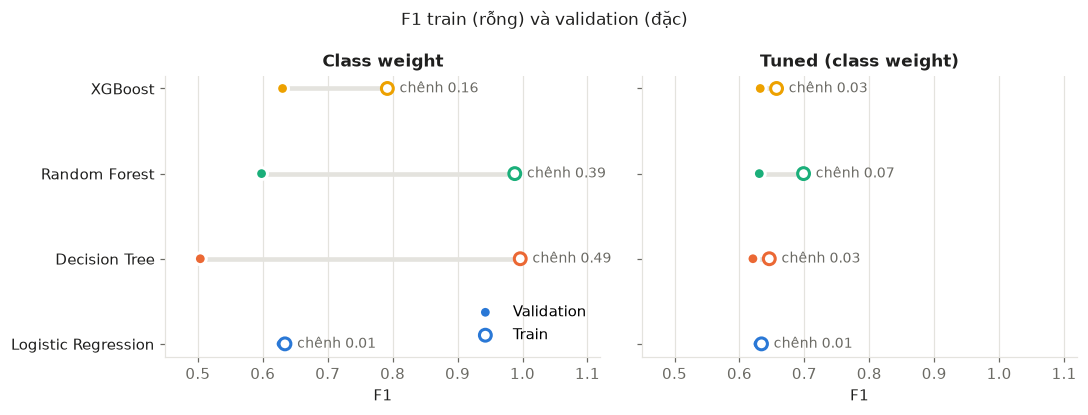
\includegraphics[width=\textwidth]{img/nb_train_val_gap.png}
\caption{F1 trên phần huấn luyện (vòng rỗng) và validation (chấm đặc) của mỗi fold, trước (trái) và sau tuning (phải)}
\label{fig:tuning_gap}
\end{figure}

\subsubsection{Phân tích}
\begin{itemize}
    \item \textbf{Tuning giải quyết được overfitting của mô hình cây.} Khoảng cách F1 train--validation giảm từ 0,49 xuống 0,03 với Decision Tree, từ 0,39 xuống 0,07 với Random Forest và từ 0,16 xuống 0,03 với XGBoost (Hình~\ref{fig:tuning_gap}). Các cấu hình được chọn đều đơn giản hơn mặc định: lá có ít nhất 11--51 mẫu, cây sâu tối đa 3--12, XGBoost dùng learning rate nhỏ (0,023).
    \item \textbf{Decision Tree hưởng lợi nhiều nhất}: PR-AUC tăng từ 0,389 lên 0,630, ROC-AUC từ 0,663 lên 0,830, cải thiện ở cả 5 fold. Random Forest tăng 0,063 PR-AUC. XGBoost tăng ít hơn (+0,018 PR-AUC) vì mặc định đã có một số cơ chế chống overfit (learning rate, chính quy hóa), nhưng vẫn cải thiện ở cả 5 fold.
    \item \textbf{Class weight giờ mới phát huy tác dụng với mô hình cây.} Recall của Decision Tree tăng từ 0,496 lên 0,799 và Random Forest từ 0,638 lên 0,776. Khi lá không còn thuần nhất, xác suất dự đoán mịn hơn và trọng số lớp mới thực sự dịch chuyển được quyết định -- giải thích vì sao ở Experiment 3, class weight gần như không tác động lên Decision Tree.
    \item \textbf{Logistic Regression không đổi} (\texttt{C=0,92} gần mặc định 1,0): mô hình vốn không overfit (khoảng cách train--validation 0,01), giới hạn của nó nằm ở dạng tuyến tính chứ không ở siêu tham số.
    \item \textbf{Sau tuning, bốn mô hình rất sát nhau} (F1 0,621--0,632, PR-AUC 0,630--0,671). XGBoost có PR-AUC và ROC-AUC cao nhất nhưng chênh lệch với Random Forest (0,004 PR-AUC) nhỏ hơn độ lệch chuẩn giữa các fold (0,02).
    \item \textbf{Lưu ý:} siêu tham số được chọn và chấm điểm trên cùng 5 fold, nên điểm sau tuning hơi lạc quan. Kết quả trên tập test (Mục~\ref{sec:final_test}) cho thấy mức lạc quan này nhỏ.
\end{itemize}

% ============================================================
\subsection{Experiment 5: Chọn ngưỡng quyết định}
% ============================================================
\textbf{Thiết kế:} với mỗi pipeline đã tuning, \texttt{src/threshold.py} chạy lại 5-fold CV trên tập train để lấy \textbf{xác suất out-of-fold}: mỗi khách hàng được dự đoán bởi mô hình không thấy khách hàng đó lúc huấn luyện. Ngưỡng được quét từ 0,05 đến 0,95 (bước 0,01) và chọn theo hai tiêu chí: tối đa F1 (ngưỡng chính) và tối đa F2 (coi Recall quan trọng gấp đôi Precision). Tập test không tham gia vào bước này.

\begin{table}[H]
\centering
\small
\resizebox{\textwidth}{!}{%
\begin{tabular}{lcccccc}
\toprule
\textbf{Mô hình} & \textbf{Ngưỡng F1} & \textbf{F1 ở 0,5} & \textbf{F1 ở ngưỡng F1} & \textbf{Fold cải thiện} & \textbf{Ngưỡng F2} & \textbf{Recall ở ngưỡng F2} \\
\midrule
Logistic Regression & 0,60 & 0,629 & 0,637 & 4/5 & 0,32 & 0,922 \\
Decision Tree & 0,60 & 0,620 & 0,628 & 3/5 & 0,26 & 0,910 \\
Random Forest & 0,60 & 0,631 & 0,639 & 4/5 & 0,34 & 0,889 \\
XGBoost & 0,57 & 0,632 & 0,639 & 3/5 & 0,37 & 0,887 \\
\bottomrule
\end{tabular}}
\caption{Ngưỡng được chọn trên xác suất out-of-fold của tập train}
\label{tab:threshold}
\end{table}

\begin{figure}[H]
\centering
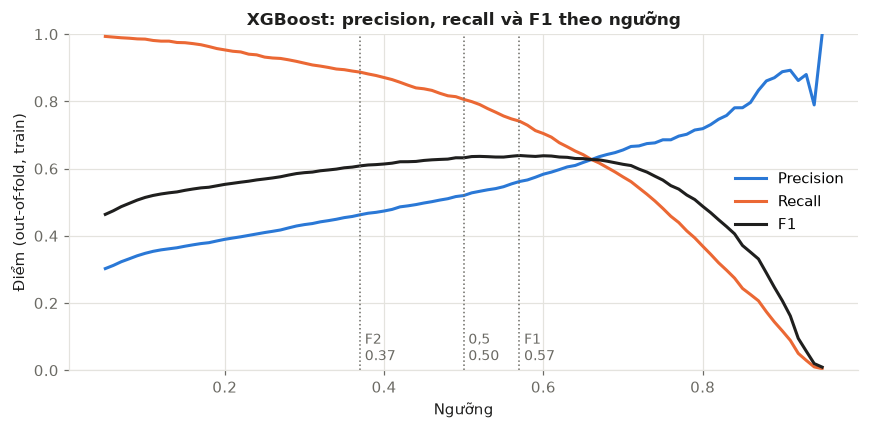
\includegraphics[width=0.8\textwidth]{img/nb_threshold_xgb.png}
\caption{Precision, Recall và F1 của XGBoost theo ngưỡng (out-of-fold trên tập train)}
\label{fig:threshold}
\end{figure}

\subsubsection{Phân tích}
\begin{itemize}
    \item \textbf{Ngưỡng tối ưu F1 cao hơn 0,5} (0,57--0,60). Class weight đã đẩy xác suất dự đoán lên cao, khiến ở ngưỡng 0,5 mô hình nghiêng hẳn về Recall (khoảng 0,80); ngưỡng tối ưu F1 kéo cân bằng ngược lại một chút về phía Precision.
    \item \textbf{Mức cải thiện F1 nhỏ} (+0,007 đến +0,008) và chỉ ở 3--4/5 fold. Đường F1 khá phẳng trong khoảng 0,45--0,65 (Hình~\ref{fig:threshold}), nên chọn ngưỡng nào trong khoảng này cũng cho F1 gần như nhau. Vai trò chính của ngưỡng là \textit{điều chỉnh cân bằng Precision--Recall} theo nhu cầu kinh doanh, không phải tăng F1.
    \item \textbf{Ngưỡng F2} (0,26--0,37) cho Recall 0,89--0,92 nhưng F1 giảm 0,02--0,05: phù hợp khi doanh nghiệp coi việc bỏ sót khách hàng rời bỏ tốn kém hơn nhiều so với gửi nhầm ưu đãi.
\end{itemize}

% ============================================================
\subsection{Kết quả cuối cùng trên tập test}\label{sec:final_test}
% ============================================================
\textbf{Chọn mô hình:} trước khi dùng tập test, nhóm chọn \textbf{XGBoost đã tuning, class weight, ngưỡng 0,57} làm mô hình chính vì có PR-AUC cross-validation cao nhất (0,671). Tập test (1.409 khách hàng, 374 rời bỏ) chỉ được dùng một lần ở bước này (\texttt{python -m src.evaluate --model-dir outputs/models/tuned}).

\begin{table}[H]
\centering
\small
\resizebox{\textwidth}{!}{%
\begin{tabular}{lcccccccc}
\toprule
\textbf{Mô hình} & \textbf{Ngưỡng} & \textbf{Precision} & \textbf{Recall} & \textbf{F1} & \textbf{F1 ở 0,5} & \textbf{ROC-AUC} & \textbf{PR-AUC} & \textbf{TP / FN / FP} \\
\midrule
\textbf{XGBoost} & 0,57 & 0,550 & \textbf{0,749} & \textbf{0,634} & 0,627 & \textbf{0,846} & \textbf{0,662} & 280 / 94 / 229 \\
Random Forest & 0,60 & \textbf{0,566} & 0,695 & 0,624 & 0,639 & 0,843 & 0,651 & 260 / 114 / 199 \\
Decision Tree & 0,60 & 0,559 & 0,719 & 0,629 & 0,627 & 0,835 & 0,624 & 269 / 105 / 212 \\
Logistic Regression & 0,60 & 0,539 & 0,706 & 0,611 & 0,614 & 0,842 & 0,633 & 264 / 110 / 226 \\
\bottomrule
\end{tabular}}
\caption{Kết quả trên tập test của các mô hình đã tuning (class weight, ngưỡng tối ưu F1)}
\label{tab:final_test}
\end{table}

\begin{figure}[H]
\centering
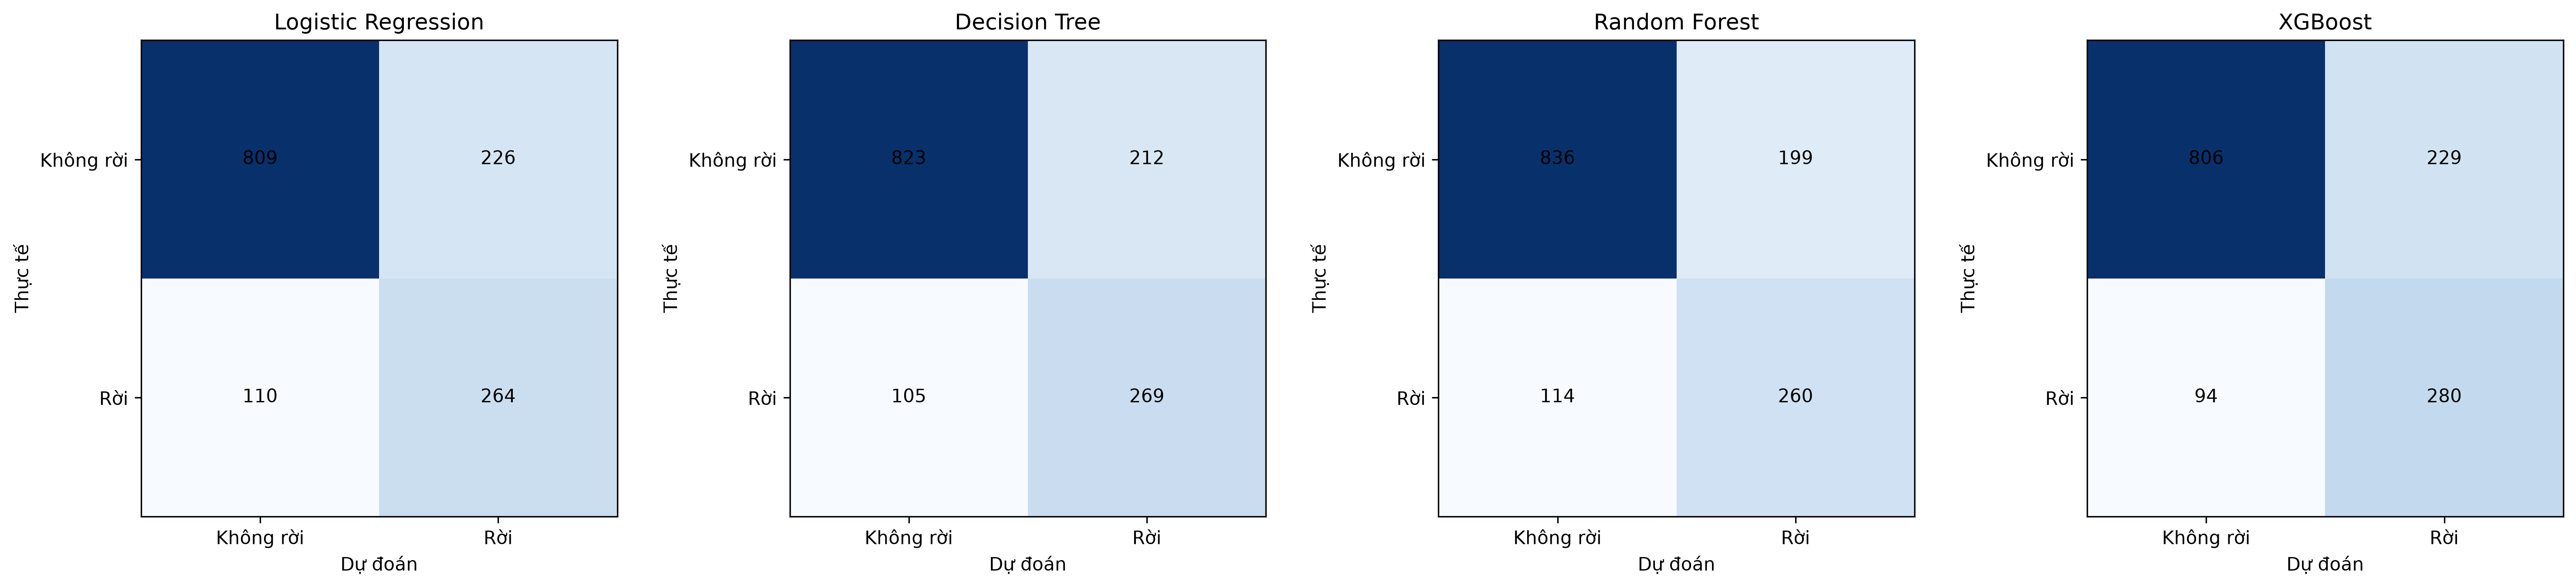
\includegraphics[width=\textwidth]{img/final_confusion.png}
\caption{Confusion Matrix trên tập test của các mô hình đã tuning với ngưỡng tối ưu F1}
\end{figure}

\begin{figure}[H]
\centering
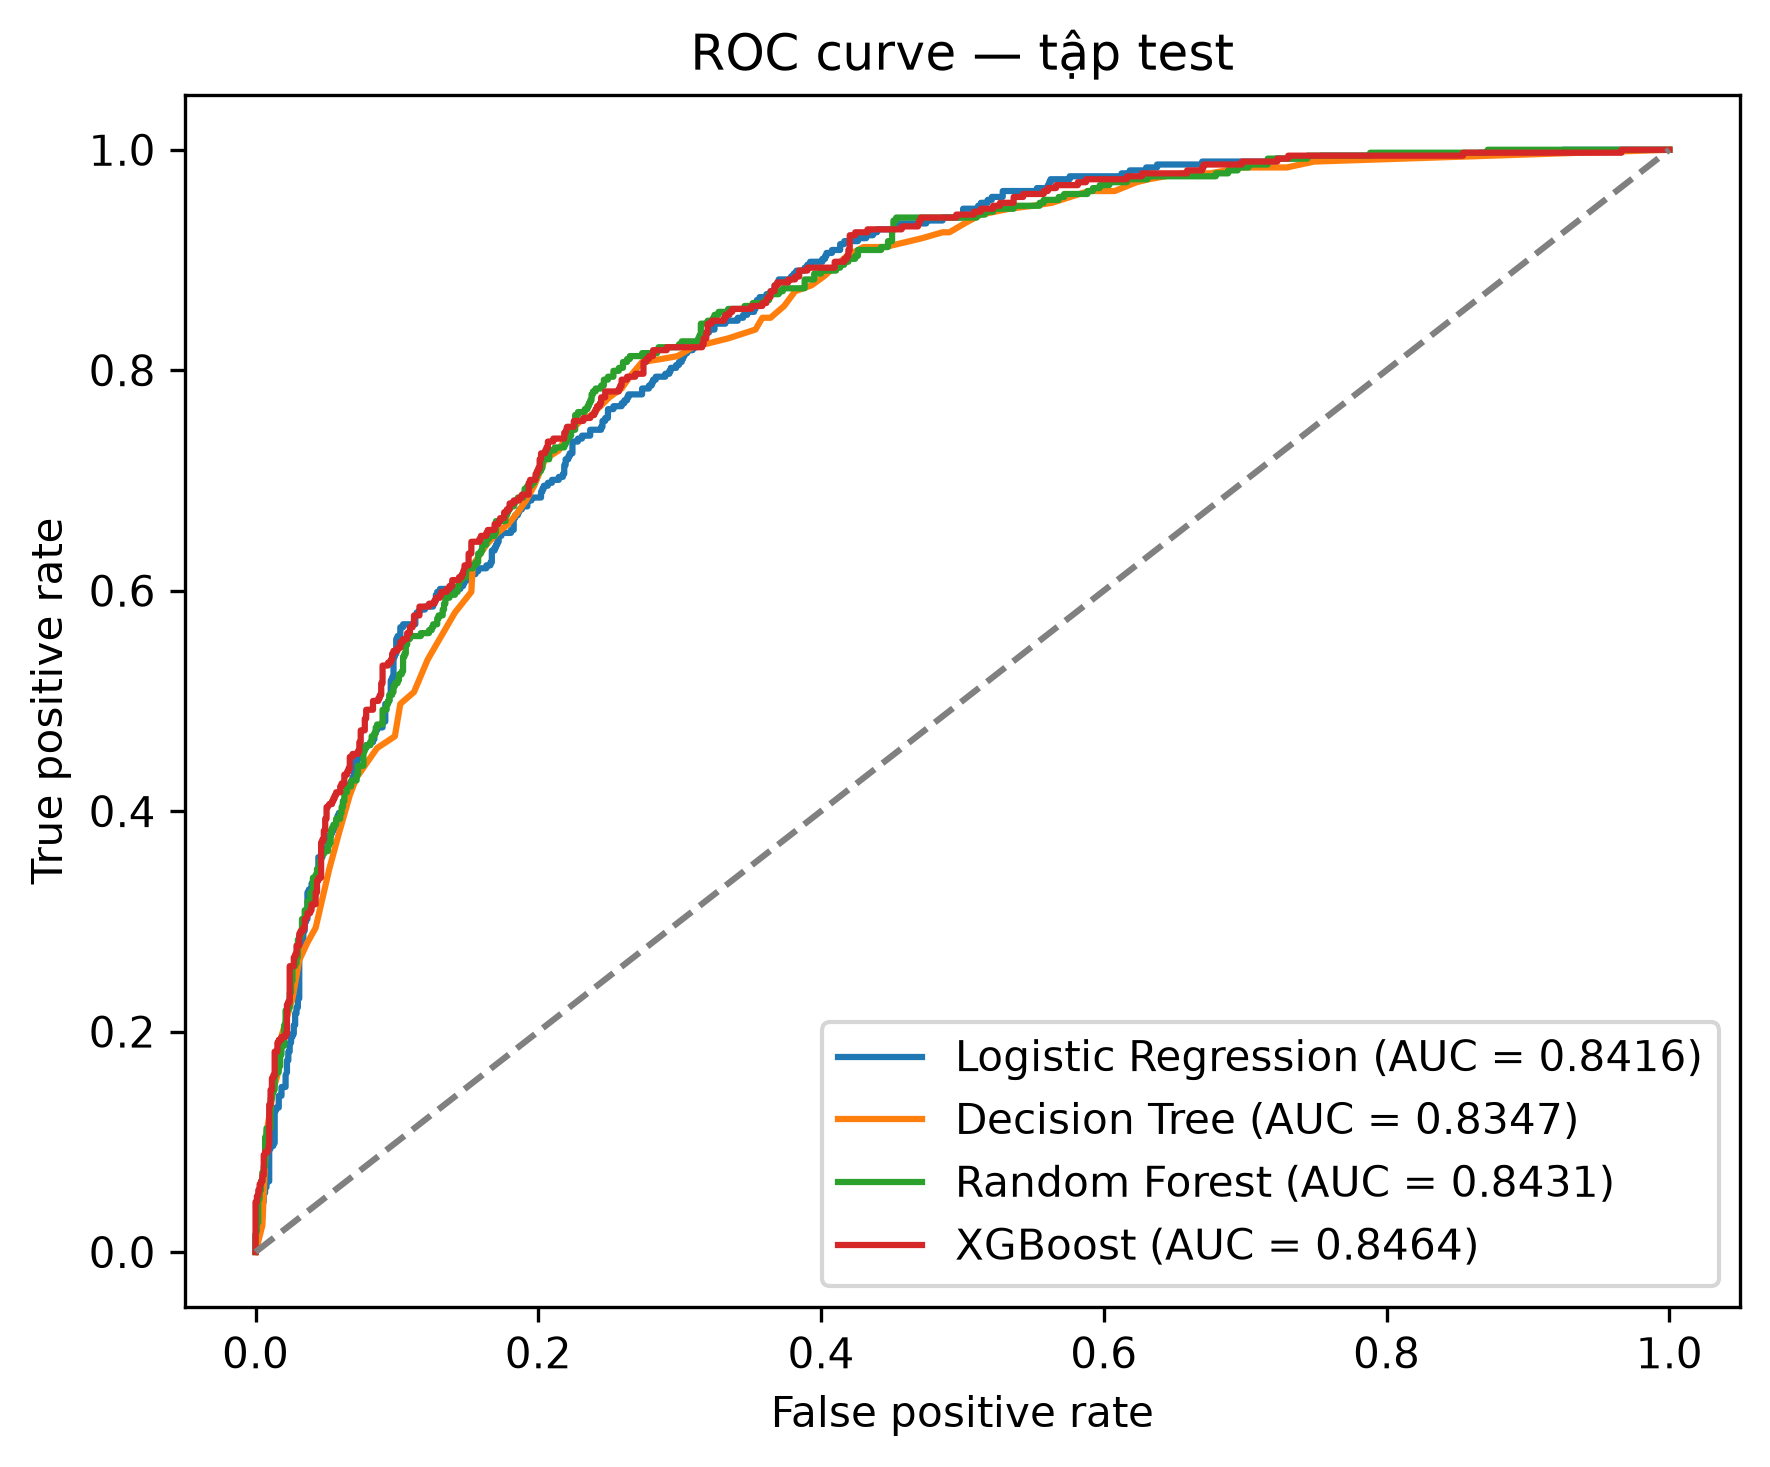
\includegraphics[width=0.49\textwidth]{img/final_roc.png}
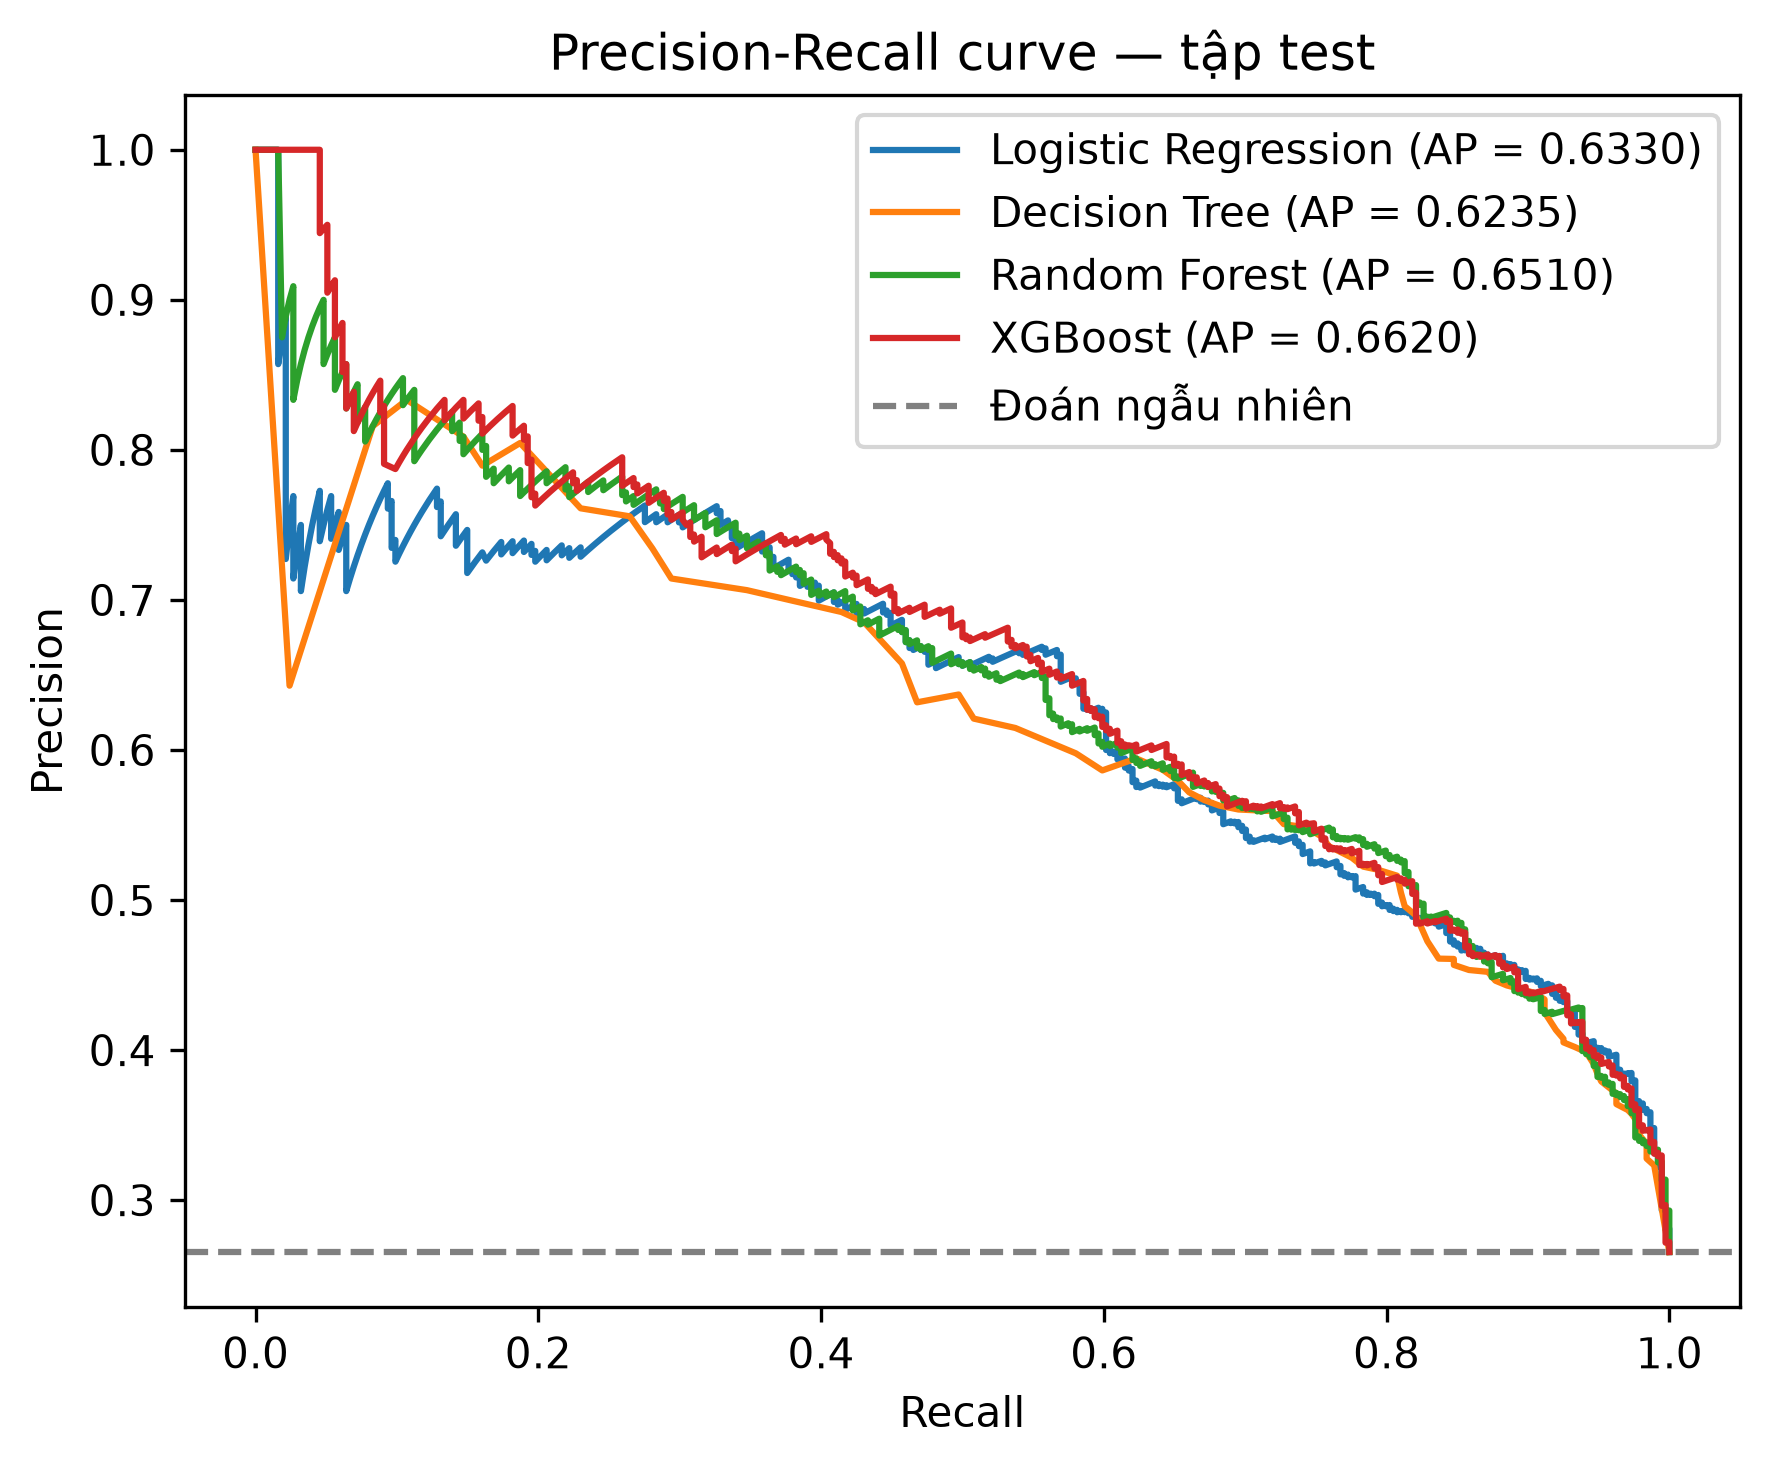
\includegraphics[width=0.49\textwidth]{img/final_pr.png}
\caption{Đường ROC (trái) và Precision--Recall (phải) trên tập test}
\end{figure}

\begin{table}[H]
\centering
\small
\resizebox{\textwidth}{!}{%
\begin{tabular}{lccccccc}
\toprule
\textbf{Mô hình} & \textbf{CV F1} & \textbf{Test F1} & \textbf{CV ROC-AUC} & \textbf{Test ROC-AUC} & \textbf{CV PR-AUC} & \textbf{Test PR-AUC} & \textbf{$\Delta$PR-AUC} \\
\midrule
Logistic Regression & 0,637 & 0,611 & 0,846 & 0,842 & 0,660 & 0,633 & $-$0,027 \\
Decision Tree & 0,628 & 0,629 & 0,830 & 0,835 & 0,630 & 0,624 & $-$0,007 \\
Random Forest & 0,639 & 0,624 & 0,848 & 0,843 & 0,667 & 0,651 & $-$0,016 \\
XGBoost & 0,639 & 0,634 & 0,850 & 0,846 & 0,671 & 0,662 & $-$0,009 \\
\bottomrule
\end{tabular}}
\caption{So sánh cross-validation và tập test (cùng ngưỡng)}
\label{tab:cv_vs_test}
\end{table}

Nhận xét:
\begin{itemize}
    \item \textbf{XGBoost đạt kết quả tốt nhất trên tập test} ở F1 (0,634), Recall (0,749), ROC-AUC (0,846) và PR-AUC (0,662), khớp với lựa chọn dựa trên cross-validation. Mô hình phát hiện được 280/374 khách hàng rời bỏ; đổi lại có 229/1.035 khách hàng ở lại bị cảnh báo nhầm.
    \item \textbf{Kết quả test khớp với cross-validation}: ROC-AUC sai khác không quá 0,005 và PR-AUC giảm 0,007--0,027 (Bảng~\ref{tab:cv_vs_test}). Mức giảm nhỏ này phản ánh độ lạc quan của việc chọn siêu tham số và ngưỡng trên cùng các fold; với XGBoost chỉ là 0,009 PR-AUC. Quy trình chọn mô hình không bị overfit vào các fold.
    \item \textbf{Chênh lệch giữa các mô hình nhỏ}: F1 của bốn mô hình nằm trong khoảng 0,611--0,634. Với 374 khách hàng rời bỏ trong tập test, chênh lệch F1 cỡ 0,02 có thể chỉ là nhiễu. Logistic Regression gần ngang bằng (ROC-AUC 0,842) và dễ giải thích hơn.
    \item \textbf{Ngưỡng tối ưu F1 trên train không đảm bảo tốt hơn 0,5 trên test}: F1 tăng với XGBoost (0,627 lên 0,634) và Decision Tree, nhưng giảm với Random Forest (0,639 xuống 0,624) và Logistic Regression. Điều này phù hợp với nhận xét ở Experiment 5 rằng đường F1 khá phẳng quanh ngưỡng tối ưu.
\end{itemize}

\textbf{Ngưỡng ưu tiên Recall (F2):} nếu dùng ngưỡng F2 (XGBoost 0,37), mô hình phát hiện 329/374 khách hàng rời bỏ (Recall 0,880) với Precision 0,460 (386 cảnh báo nhầm), F1 0,604. Đây là lựa chọn phù hợp khi chi phí của một ưu đãi thấp so với giá trị của khách hàng giữ lại được.

\textbf{So với lần đánh giá test đầu tiên} (Decision Tree và Random Forest với tham số mặc định, không xử lý mất cân bằng, ngưỡng 0,5): F1 của Decision Tree tăng từ 0,492 lên 0,629 (Recall 0,497 lên 0,719, ROC-AUC 0,654 lên 0,835); Random Forest tăng từ 0,544 lên 0,624 (Recall 0,481 lên 0,695, ROC-AUC 0,821 lên 0,843).

% ============================================================
\subsection{Giải thích mô hình}
% ============================================================

\subsubsection{Permutation importance}
Với mỗi đặc trưng gốc, nhóm xáo trộn ngẫu nhiên giá trị của nó trên tập test (20 lần) và đo mức giảm PR-AUC. Cách này áp dụng được cho mọi mô hình và làm việc trên 19 đặc trưng gốc (không phải các cột one-hot), nên dễ diễn giải.

\begin{figure}[H]
\centering
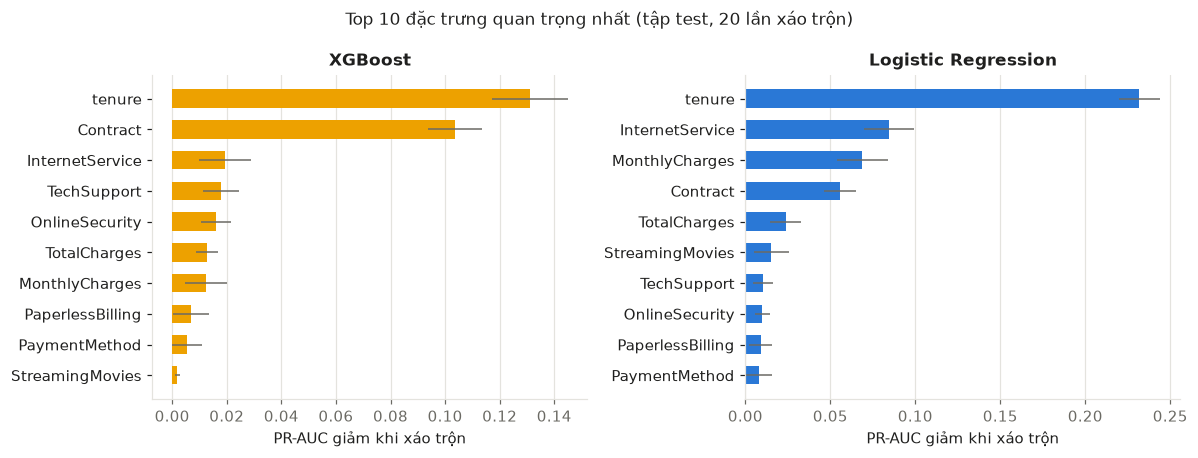
\includegraphics[width=\textwidth]{img/nb_permutation_importance.png}
\caption{Permutation importance trên tập test: mức giảm PR-AUC khi xáo trộn từng đặc trưng (10 đặc trưng quan trọng nhất; vạch: độ lệch chuẩn qua 20 lần xáo trộn)}
\label{fig:perm}
\end{figure}

\begin{table}[H]
\centering
\small
\begin{tabular}{lcc}
\toprule
\textbf{Đặc trưng} & \textbf{XGBoost} & \textbf{Logistic Regression} \\
\midrule
\texttt{tenure} & \textbf{0,131} & \textbf{0,232} \\
\texttt{Contract} & 0,104 & 0,056 \\
\texttt{InternetService} & 0,019 & 0,084 \\
\texttt{TechSupport} & 0,018 & 0,010 \\
\texttt{OnlineSecurity} & 0,016 & 0,010 \\
\texttt{TotalCharges} & 0,013 & 0,024 \\
\texttt{MonthlyCharges} & 0,012 & 0,069 \\
\texttt{PaperlessBilling} & 0,007 & 0,009 \\
\texttt{PaymentMethod} & 0,005 & 0,008 \\
\bottomrule
\end{tabular}
\caption{Mức giảm PR-AUC trên tập test khi xáo trộn từng đặc trưng}
\end{table}

\subsubsection{Hệ số Logistic Regression}
Hệ số dương làm tăng khả năng rời bỏ, hệ số âm làm giảm. Tỉ số odds $e^{\beta}$ cho biết odds rời bỏ thay đổi bao nhiêu lần khi khách hàng thuộc nhóm đó (biến one-hot) hoặc khi đặc trưng tăng một độ lệch chuẩn (biến số đã chuẩn hóa).

\begin{table}[H]
\centering
\small
\begin{tabular}{lcc@{\hskip 1.2cm}lcc}
\toprule
\multicolumn{3}{c}{\textbf{Tăng khả năng rời bỏ}} & \multicolumn{3}{c}{\textbf{Giảm khả năng rời bỏ}} \\
\cmidrule(lr){1-3} \cmidrule(lr){4-6}
\textbf{Đặc trưng} & $\beta$ & $e^{\beta}$ & \textbf{Đặc trưng} & $\beta$ & $e^{\beta}$ \\
\midrule
InternetService = Fiber optic & 0,686 & 1,98 & \texttt{tenure} & $-$1,151 & 0,32 \\
Contract = Month-to-month & 0,656 & 1,93 & Contract = Two year & $-$0,774 & 0,46 \\
\texttt{TotalCharges} & 0,484 & 1,62 & \texttt{MonthlyCharges} & $-$0,632 & 0,53 \\
StreamingMovies = Yes & 0,265 & 1,30 & InternetService = DSL & $-$0,609 & 0,54 \\
StreamingTV = Yes & 0,251 & 1,29 & InternetService = No & $-$0,268 & 0,77 \\
PaymentMethod = Electronic check & 0,240 & 1,27 & & & \\
OnlineSecurity = No & 0,199 & 1,22 & & & \\
TechSupport = No & 0,165 & 1,18 & & & \\
\bottomrule
\end{tabular}
\caption{Các hệ số lớn nhất của Logistic Regression đã tuning}
\end{table}

\subsubsection{Nhận xét}
\begin{itemize}
    \item \textbf{\texttt{tenure} là đặc trưng quan trọng nhất} với cả hai mô hình: khách hàng càng gắn bó lâu càng ít rời bỏ (mỗi độ lệch chuẩn \texttt{tenure}, khoảng 24 tháng, làm odds rời bỏ giảm còn 0,32 lần).
    \item \textbf{\texttt{Contract}} đứng thứ hai với XGBoost: hợp đồng theo tháng làm odds rời bỏ tăng gần gấp đôi, hợp đồng 2 năm làm giảm còn khoảng một nửa.
    \item \textbf{\texttt{InternetService}}: Fiber optic làm tăng nguy cơ rời bỏ, DSL làm giảm. Các \textbf{dịch vụ hỗ trợ} (\texttt{TechSupport}, \texttt{OnlineSecurity}) và \textbf{thanh toán bằng Electronic check} cũng làm tăng nguy cơ.
    \item Các đặc trưng nhân khẩu học (giới tính, có vợ/chồng, người phụ thuộc) không có mặt trong nhóm quan trọng nhất. Kết quả thống nhất với các quan sát trong phần EDA (Mục~\ref{sec:eda}).
    \item \textbf{Lưu ý về đa cộng tuyến:} \texttt{TotalCharges} xấp xỉ \texttt{tenure} $\times$ \texttt{MonthlyCharges}, nên ba biến này tương quan mạnh với nhau. Dấu hệ số của từng biến riêng lẻ (\texttt{MonthlyCharges} âm, \texttt{TotalCharges} dương) không nên diễn giải tách rời. Permutation importance đáng tin cậy hơn để đánh giá mức độ quan trọng, nhưng cũng có thể đánh giá thấp các đặc trưng tương quan với nhau. Các giải thích này là quan hệ thống kê mà mô hình học được, không phải quan hệ nhân quả.
\end{itemize}

% ============================================================
\subsection{Tổng hợp kết quả}
% ============================================================

\begin{figure}[H]
\centering
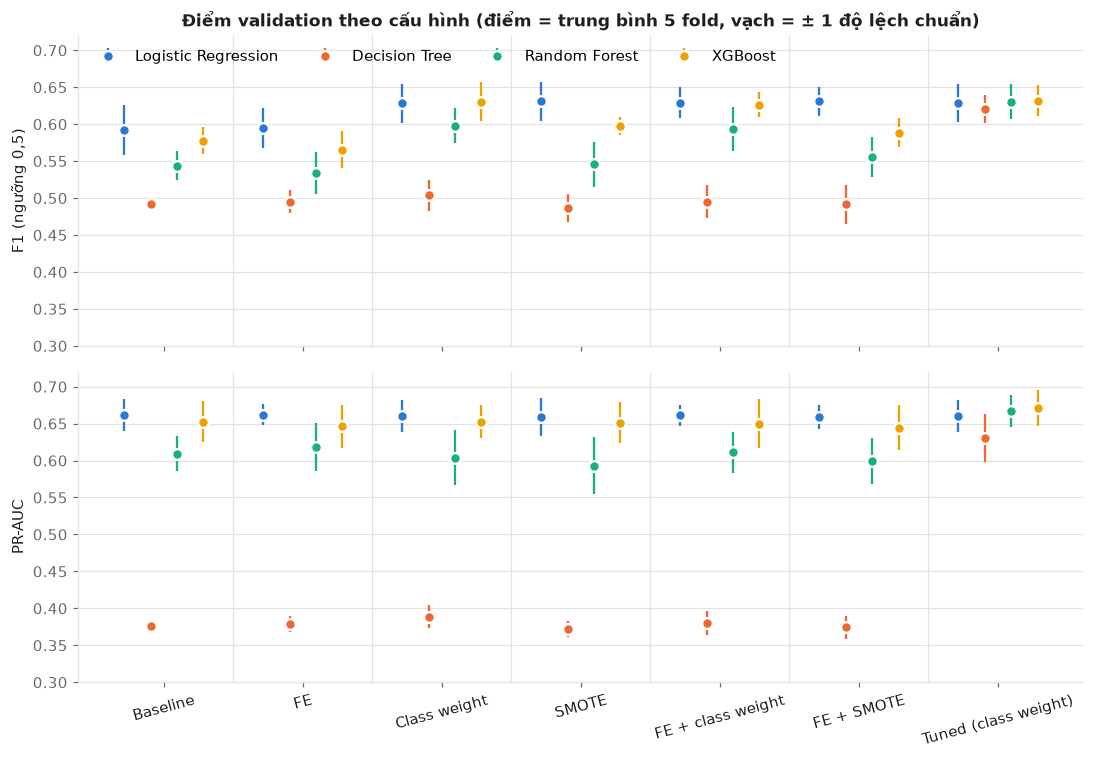
\includegraphics[width=\textwidth]{img/nb_cv_overview.png}
\caption{F1 (ngưỡng 0,5) và PR-AUC validation của mọi cấu hình (chấm: trung bình 5 fold; vạch: $\pm$ 1 độ lệch chuẩn)}
\label{fig:cv_overview}
\end{figure}

\begin{table}[H]
\centering
\small
\begin{tabular}{l c p{9cm}}
\toprule
\textbf{Thay đổi} & \textbf{Tác động} & \textbf{Ghi chú} \\
\midrule
Class weight & \textbf{Lớn} & F1 +0,036 đến +0,054 với LR, RF, XGBoost (5/5 fold); Recall tăng 0,16--0,26; đổi lại Precision giảm. \\
SMOTE & Trung bình & Tương đương class weight với LR; yếu hơn với mô hình cây. Class weight đơn giản hơn và không sinh dữ liệu giả. \\
Tuning & \textbf{Lớn với mô hình cây} & Decision Tree: F1 +0,12, PR-AUC +0,24; Random Forest: F1 +0,03, PR-AUC +0,06; nhờ giới hạn độ sâu và kích thước lá, giảm overfit. Không đổi với LR. \\
Feature Engineering & Không đáng kể & Mọi chênh lệch trong khoảng $\pm 0{,}012$, nhỏ hơn độ dao động giữa các fold. \\
Chọn ngưỡng & Nhỏ với F1 & +0,008 F1 trên CV, trên test lúc tăng lúc giảm. Chủ yếu dùng để điều chỉnh cân bằng Precision--Recall. \\
\bottomrule
\end{tabular}
\caption{Tác động của từng kỹ thuật}
\label{tab:summary_effects}
\end{table}

Hình~\ref{fig:cv_overview} và Bảng~\ref{tab:summary_effects} cho thấy hai kỹ thuật mang lại cải thiện chính là \textbf{xử lý mất cân bằng bằng class weight} (giải quyết Recall thấp) và \textbf{tuning} (giải quyết overfitting của mô hình cây). Sau khi kết hợp hai kỹ thuật này, bốn mô hình đạt hiệu năng rất sát nhau, cho thấy giới hạn hiện tại nằm ở thông tin có trong dữ liệu hơn là ở lựa chọn thuật toán.

\section{Kết luận và hướng phát triển}

\subsection{Kết quả đạt được}
\begin{itemize}
    \item Xây dựng được pipeline học máy hoàn chỉnh và có thể tái lập cho bài toán dự đoán khách hàng rời bỏ: làm sạch dữ liệu có kiểm tra, tiền xử lý bằng \texttt{ColumnTransformer}, Feature Engineering, xử lý mất cân bằng, cross-validation phân tầng, tuning siêu tham số, chọn ngưỡng quyết định, đánh giá trên tập test và dự đoán cho khách hàng mới.
    \item Quy trình đánh giá được thiết kế để tránh rò rỉ dữ liệu: tập test được tách riêng từ đầu và chỉ dùng một lần; mọi bước tiền xử lý, Feature Engineering và SMOTE nằm trong Pipeline nên chỉ được \texttt{fit} trên phần huấn luyện của từng fold; ngưỡng được chọn trên xác suất out-of-fold của tập train; mọi thực nghiệm dùng chung 5 fold nên so sánh được theo cặp.
    \item Ở cấu hình baseline, Logistic Regression tốt nhất (F1 0,592, ROC-AUC 0,846, PR-AUC 0,662), sát sau là XGBoost; Decision Tree và Random Forest overfit nặng. Recall của mọi mô hình chỉ khoảng 0,48--0,54.
    \item \textbf{Class weight} giải quyết được vấn đề Recall thấp: F1 tăng 0,036--0,054 ở cả 5 fold với Logistic Regression, Random Forest và XGBoost, Recall tăng 0,16--0,26. SMOTE chỉ tương đương với Logistic Regression và kém hơn với mô hình cây.
    \item \textbf{Tuning} bằng RandomizedSearchCV giải quyết overfitting của mô hình cây: khoảng cách F1 train--validation giảm từ 0,16--0,49 xuống 0,03--0,07; PR-AUC của Decision Tree tăng 0,24, Random Forest tăng 0,06.
    \item \textbf{Feature Engineering} (9 đặc trưng mới) và \textbf{chọn ngưỡng} gần như không thay đổi F1: chênh lệch nằm trong mức dao động giữa các fold.
    \item Mô hình cuối cùng là \textbf{XGBoost đã tuning, class weight, ngưỡng 0,57}, được chọn trước khi dùng tập test dựa trên PR-AUC cross-validation cao nhất (0,671). Trên tập test, mô hình đạt F1 0,634, Recall 0,749, Precision 0,550, ROC-AUC 0,846, PR-AUC 0,662 và phát hiện được 280/374 khách hàng rời bỏ. Kết quả test khớp với cross-validation (PR-AUC 0,671 so với 0,662).
    \item Permutation importance và hệ số Logistic Regression thống nhất với EDA: \texttt{tenure}, \texttt{Contract}, \texttt{InternetService}, các dịch vụ hỗ trợ (\texttt{TechSupport}, \texttt{OnlineSecurity}) và phương thức thanh toán là các yếu tố quan trọng nhất.
\end{itemize}

\subsection{Kết luận chung}
Hai kỹ thuật mang lại cải thiện chính là xử lý mất cân bằng bằng class weight và tuning siêu tham số; Feature Engineering và chọn ngưỡng chỉ có tác động nhỏ. Sau khi áp dụng cả hai kỹ thuật chính, bốn mô hình đạt hiệu năng rất sát nhau (F1 test 0,611--0,634). Với 374 khách hàng rời bỏ trong tập test, chênh lệch cỡ 0,02 có thể chỉ là nhiễu, nên Logistic Regression -- đơn giản, nhanh và dễ giải thích -- vẫn là một lựa chọn thay thế đáng cân nhắc.

\subsection{Ý nghĩa kinh doanh}
Các quan sát từ dữ liệu gợi ý một số hướng hành động cho doanh nghiệp, với lưu ý đây là mối liên hệ thống kê, không phải quan hệ nhân quả:
\begin{itemize}
    \item Khách hàng hợp đồng theo tháng, mới sử dụng dịch vụ (\texttt{tenure} thấp) là nhóm rủi ro cao nhất; ưu đãi chuyển sang hợp đồng dài hạn có thể là đòn bẩy giữ chân.
    \item Khách hàng dùng Fiber optic nhưng không đăng ký TechSupport/OnlineSecurity có tỉ lệ rời bỏ cao; cần xem xét chất lượng dịch vụ và gói hỗ trợ đi kèm.
    \item Mô hình xuất ra xác suất rời bỏ cho phép xếp hạng khách hàng và ưu tiên nguồn lực chăm sóc. Ngưỡng quyết định nên được chọn theo chi phí: ngưỡng tối ưu F1 (0,57) cân bằng Precision và Recall; nếu bỏ sót một khách hàng rời bỏ tốn kém hơn nhiều so với gửi nhầm một ưu đãi, ngưỡng F2 (0,37) phát hiện được 329/374 khách hàng rời bỏ với Precision 0,46.
\end{itemize}

\subsection{Hạn chế và hướng phát triển}
\begin{itemize}
    \item Bộ dữ liệu là ảnh chụp tĩnh tại một thời điểm, không có thông tin hành vi theo thời gian (số cuộc gọi hỗ trợ, lịch sử thanh toán trễ,\ldots).
    \item Kích thước dữ liệu nhỏ (7.043 khách hàng) nên chênh lệch giữa các mô hình tốt nhất thường nằm trong mức dao động giữa các fold.
    \item Siêu tham số và ngưỡng được chọn trên cùng các fold dùng để chấm điểm, nên điểm cross-validation sau tuning hơi lạc quan; nested cross-validation sẽ cho ước lượng khách quan hơn (tập test cho thấy mức lạc quan này nhỏ).
    \item Chưa thực hiện so sánh các phương pháp Encoding/Scaling như kế hoạch ban đầu.
    \item Hướng phát triển: chọn ngưỡng theo hàm chi phí khi có số liệu kinh doanh, hiệu chỉnh xác suất (\textit{probability calibration}), giải thích theo từng khách hàng bằng SHAP, thử thêm LightGBM/CatBoost, và triển khai mô hình dưới dạng API hoặc dashboard.
\end{itemize}

\begin{thebibliography}{99}

\bibitem{huang2012}
B.~Huang, M.~T. Kechadi, and B.~Buckley,
``Customer churn prediction in telecommunications,''
\textit{Expert Systems with Applications}, vol.~39, no.~1, pp.~1414--1425, 2012.

\bibitem{verbeke2012}
W.~Verbeke, K.~Dejaeger, D.~Martens, J.~Hur, and B.~Baesens,
``New insights into churn prediction in the telecommunication sector: A profit driven data mining approach,''
\textit{European Journal of Operational Research}, vol.~218, no.~1, pp.~211--229, 2012.

\bibitem{vafeiadis2015}
T.~Vafeiadis, K.~I. Diamantaras, G.~Sarigiannidis, and K.~C. Chatzisavvas,
``A comparison of machine learning techniques for customer churn prediction,''
\textit{Simulation Modelling Practice and Theory}, vol.~55, pp.~1--9, 2015.

\bibitem{ahmad2019}
A.~K. Ahmad, A.~Jafar, and K.~Aljoumaa,
``Customer churn prediction in telecom using machine learning in big data platform,''
\textit{Journal of Big Data}, vol.~6, no.~28, 2019.

\bibitem{hosmer2013}
D.~W. Hosmer, S.~Lemeshow, and R.~X. Sturdivant,
\textit{Applied Logistic Regression}, 3rd~ed. Wiley, 2013.

\bibitem{breiman1984}
L.~Breiman, J.~Friedman, R.~Olshen, and C.~Stone,
\textit{Classification and Regression Trees}. Wadsworth, 1984.

\bibitem{breiman2001}
L.~Breiman,
``Random forests,''
\textit{Machine Learning}, vol.~45, no.~1, pp.~5--32, 2001.

\bibitem{chen2016}
T.~Chen and C.~Guestrin,
``XGBoost: A scalable tree boosting system,''
in \textit{Proc. 22nd ACM SIGKDD Int. Conf. on Knowledge Discovery and Data Mining}, 2016, pp.~785--794.

\bibitem{chawla2002}
N.~V. Chawla, K.~W. Bowyer, L.~O. Hall, and W.~P. Kegelmeyer,
``SMOTE: Synthetic minority over-sampling technique,''
\textit{Journal of Artificial Intelligence Research}, vol.~16, pp.~321--357, 2002.

\bibitem{bergstra2012}
J.~Bergstra and Y.~Bengio,
``Random search for hyper-parameter optimization,''
\textit{Journal of Machine Learning Research}, vol.~13, pp.~281--305, 2012.

\bibitem{akiba2019}
T.~Akiba, S.~Sano, T.~Yanase, T.~Ohta, and M.~Koyama,
``Optuna: A next-generation hyperparameter optimization framework,''
in \textit{Proc. 25th ACM SIGKDD Int. Conf. on Knowledge Discovery and Data Mining}, 2019, pp.~2623--2631.

\bibitem{lundberg2017}
S.~M. Lundberg and S.-I. Lee,
``A unified approach to interpreting model predictions,''
in \textit{Advances in Neural Information Processing Systems 30}, 2017.

\bibitem{pedregosa2011}
F.~Pedregosa \textit{et al.},
``Scikit-learn: Machine learning in Python,''
\textit{Journal of Machine Learning Research}, vol.~12, pp.~2825--2830, 2011.

\bibitem{kaggle_telco}
IBM Sample Data Sets, ``Telco Customer Churn,'' Kaggle.
\url{https://www.kaggle.com/datasets/blastchar/telco-customer-churn}

\end{thebibliography}

\end{document}
